% Options for packages loaded elsewhere
\PassOptionsToPackage{unicode}{hyperref}
\PassOptionsToPackage{hyphens}{url}
\documentclass[
]{article}
\usepackage{xcolor}
\usepackage{amsmath,amssymb}
\setcounter{secnumdepth}{-\maxdimen} % remove section numbering
\usepackage{iftex}
\ifPDFTeX
  \usepackage[T1]{fontenc}
  \usepackage[utf8]{inputenc}
  \usepackage{textcomp} % provide euro and other symbols
\else % if luatex or xetex
  \usepackage{unicode-math} % this also loads fontspec
  \defaultfontfeatures{Scale=MatchLowercase}
  \defaultfontfeatures[\rmfamily]{Ligatures=TeX,Scale=1}
\fi
\usepackage{lmodern}
\ifPDFTeX\else
  % xetex/luatex font selection
\fi
% Use upquote if available, for straight quotes in verbatim environments
\IfFileExists{upquote.sty}{\usepackage{upquote}}{}
\IfFileExists{microtype.sty}{% use microtype if available
  \usepackage[]{microtype}
  \UseMicrotypeSet[protrusion]{basicmath} % disable protrusion for tt fonts
}{}
\makeatletter
\@ifundefined{KOMAClassName}{% if non-KOMA class
  \IfFileExists{parskip.sty}{%
    \usepackage{parskip}
  }{% else
    \setlength{\parindent}{0pt}
    \setlength{\parskip}{6pt plus 2pt minus 1pt}}
}{% if KOMA class
  \KOMAoptions{parskip=half}}
\makeatother
\usepackage{color}
\usepackage{fancyvrb}
\newcommand{\VerbBar}{|}
\newcommand{\VERB}{\Verb[commandchars=\\\{\}]}
\DefineVerbatimEnvironment{Highlighting}{Verbatim}{commandchars=\\\{\}}
% Add ',fontsize=\small' for more characters per line
\newenvironment{Shaded}{}{}
\newcommand{\AlertTok}[1]{\textcolor[rgb]{1.00,0.00,0.00}{\textbf{#1}}}
\newcommand{\AnnotationTok}[1]{\textcolor[rgb]{0.38,0.63,0.69}{\textbf{\textit{#1}}}}
\newcommand{\AttributeTok}[1]{\textcolor[rgb]{0.49,0.56,0.16}{#1}}
\newcommand{\BaseNTok}[1]{\textcolor[rgb]{0.25,0.63,0.44}{#1}}
\newcommand{\BuiltInTok}[1]{\textcolor[rgb]{0.00,0.50,0.00}{#1}}
\newcommand{\CharTok}[1]{\textcolor[rgb]{0.25,0.44,0.63}{#1}}
\newcommand{\CommentTok}[1]{\textcolor[rgb]{0.38,0.63,0.69}{\textit{#1}}}
\newcommand{\CommentVarTok}[1]{\textcolor[rgb]{0.38,0.63,0.69}{\textbf{\textit{#1}}}}
\newcommand{\ConstantTok}[1]{\textcolor[rgb]{0.53,0.00,0.00}{#1}}
\newcommand{\ControlFlowTok}[1]{\textcolor[rgb]{0.00,0.44,0.13}{\textbf{#1}}}
\newcommand{\DataTypeTok}[1]{\textcolor[rgb]{0.56,0.13,0.00}{#1}}
\newcommand{\DecValTok}[1]{\textcolor[rgb]{0.25,0.63,0.44}{#1}}
\newcommand{\DocumentationTok}[1]{\textcolor[rgb]{0.73,0.13,0.13}{\textit{#1}}}
\newcommand{\ErrorTok}[1]{\textcolor[rgb]{1.00,0.00,0.00}{\textbf{#1}}}
\newcommand{\ExtensionTok}[1]{#1}
\newcommand{\FloatTok}[1]{\textcolor[rgb]{0.25,0.63,0.44}{#1}}
\newcommand{\FunctionTok}[1]{\textcolor[rgb]{0.02,0.16,0.49}{#1}}
\newcommand{\ImportTok}[1]{\textcolor[rgb]{0.00,0.50,0.00}{\textbf{#1}}}
\newcommand{\InformationTok}[1]{\textcolor[rgb]{0.38,0.63,0.69}{\textbf{\textit{#1}}}}
\newcommand{\KeywordTok}[1]{\textcolor[rgb]{0.00,0.44,0.13}{\textbf{#1}}}
\newcommand{\NormalTok}[1]{#1}
\newcommand{\OperatorTok}[1]{\textcolor[rgb]{0.40,0.40,0.40}{#1}}
\newcommand{\OtherTok}[1]{\textcolor[rgb]{0.00,0.44,0.13}{#1}}
\newcommand{\PreprocessorTok}[1]{\textcolor[rgb]{0.74,0.48,0.00}{#1}}
\newcommand{\RegionMarkerTok}[1]{#1}
\newcommand{\SpecialCharTok}[1]{\textcolor[rgb]{0.25,0.44,0.63}{#1}}
\newcommand{\SpecialStringTok}[1]{\textcolor[rgb]{0.73,0.40,0.53}{#1}}
\newcommand{\StringTok}[1]{\textcolor[rgb]{0.25,0.44,0.63}{#1}}
\newcommand{\VariableTok}[1]{\textcolor[rgb]{0.10,0.09,0.49}{#1}}
\newcommand{\VerbatimStringTok}[1]{\textcolor[rgb]{0.25,0.44,0.63}{#1}}
\newcommand{\WarningTok}[1]{\textcolor[rgb]{0.38,0.63,0.69}{\textbf{\textit{#1}}}}
\usepackage{graphicx}
\makeatletter
\newsavebox\pandoc@box
\newcommand*\pandocbounded[1]{% scales image to fit in text height/width
  \sbox\pandoc@box{#1}%
  \Gscale@div\@tempa{\textheight}{\dimexpr\ht\pandoc@box+\dp\pandoc@box\relax}%
  \Gscale@div\@tempb{\linewidth}{\wd\pandoc@box}%
  \ifdim\@tempb\p@<\@tempa\p@\let\@tempa\@tempb\fi% select the smaller of both
  \ifdim\@tempa\p@<\p@\scalebox{\@tempa}{\usebox\pandoc@box}%
  \else\usebox{\pandoc@box}%
  \fi%
}
% Set default figure placement to htbp
\def\fps@figure{htbp}
\makeatother
\ifLuaTeX
\usepackage[bidi=basic]{babel}
\else
\usepackage[bidi=default]{babel}
\fi
\babelprovide[main,import]{french}
% get rid of language-specific shorthands (see #6817):
\let\LanguageShortHands\languageshorthands
\def\languageshorthands#1{}
\setlength{\emergencystretch}{3em} % prevent overfull lines
\providecommand{\tightlist}{%
  \setlength{\itemsep}{0pt}\setlength{\parskip}{0pt}}
\usepackage{bookmark}
\IfFileExists{xurl.sty}{\usepackage{xurl}}{} % add URL line breaks if available
\urlstyle{same}
\hypersetup{
  pdftitle={3~ Réhaussement et visualisation d'images -- Traitement d\textquotesingle images satellites avec Python},
  pdflang={fr},
  hidelinks,
  pdfcreator={LaTeX via pandoc}}

\title{3~ Réhaussement et visualisation d'images -- Traitement
d\textquotesingle images satellites avec Python}
\author{}
\date{}

\begin{document}
\maketitle

\phantomsection\label{quarto-document-content}
\phantomsection\label{title-block-header}
\section{\texorpdfstring{\protect\hypertarget{sec-chap02}{}{{3}~
{Réhaussement et visualisation
d'images}}}{3~ Réhaussement et visualisation d'images}}\label{ruxe9haussement-et-visualisation-dimages}

Assurez-vous de lire ce préambule avant d'exécutez le reste du notebook.

\subsection{\texorpdfstring{{3.1}
Préambule}{3.1 Préambule}}\label{pruxe9ambule}

\subsubsection{\texorpdfstring{{3.1.1}
Objectifs}{3.1.1 Objectifs}}\label{objectifs}

Dans ce chapitre, nous abordons quelques techniques de réhaussement et
de visualisation d'images. Ce chapitre est aussi disponible sous la
forme d'un notebook Python:

\href{https://colab.research.google.com/github/sfoucher/TraitementImagesPythonVol1/blob/main/notebooks/02-RehaussementVisualisationImages.ipynb}{\pandocbounded{
\includegraphics[keepaspectratio]{images/colab.png}}}

\subsubsection{\texorpdfstring{{3.1.2}
Librairies}{3.1.2 Librairies}}\label{librairies}

Les librairies qui vont être explorées dans ce chapitre sont les
suivantes:

\begin{itemize}
\item
  \href{https://scipy.org/}{SciPy}
\item
  \href{https://numpy.org/}{NumPy}
\item
  \href{https://pypi.org/project/opencv-python/}{opencv-python · PyPI}
\item
  \href{https://scikit-image.org/}{scikit-image}
\item
  \href{https://rasterio.readthedocs.io/en/stable/}{Rasterio}
\item
  \href{https://docs.xarray.dev/en/stable/}{Xarray}
\item
  \href{https://corteva.github.io/rioxarray/stable/index.html}{rioxarray}
\end{itemize}

Dans l'environnement Google Colab, seul \texttt{rioxarray} et GDAL
doivent être installés:

\phantomsection\label{c4347da7}
\phantomsection\label{cb1}
\begin{Shaded}
\begin{Highlighting}[]
\OperatorTok{\%\%}\NormalTok{capture}
\OperatorTok{!}\NormalTok{apt}\OperatorTok{{-}}\NormalTok{get update}
\OperatorTok{!}\NormalTok{apt}\OperatorTok{{-}}\NormalTok{get install gdal}\OperatorTok{{-}}\BuiltInTok{bin}\NormalTok{ libgdal}\OperatorTok{{-}}\NormalTok{dev}
\OperatorTok{!}\NormalTok{pip install }\OperatorTok{{-}}\NormalTok{q rioxarray}
\OperatorTok{!}\NormalTok{pip install }\OperatorTok{{-}}\NormalTok{qU }\StringTok{"geemap[workshop]"}
\end{Highlighting}
\end{Shaded}

Dans l'environnement Google Colab, on peut s'assurer que les librairies
sont installées:

\phantomsection\label{23ee82f2}
\phantomsection\label{cb2}
\begin{Shaded}
\begin{Highlighting}[]
\OperatorTok{\%\%}\NormalTok{capture}
\OperatorTok{!}\NormalTok{pip install }\OperatorTok{{-}}\NormalTok{qU matplotlib rioxarray xrscipy scikit}\OperatorTok{{-}}\NormalTok{image}
\end{Highlighting}
\end{Shaded}

Vérifier les importations:

\phantomsection\label{cfa89116}
\phantomsection\label{cb3}
\begin{Shaded}
\begin{Highlighting}[]
\ImportTok{import}\NormalTok{ numpy }\ImportTok{as}\NormalTok{ np}
\ImportTok{import}\NormalTok{ rioxarray }\ImportTok{as}\NormalTok{ rxr}
\ImportTok{from}\NormalTok{ scipy }\ImportTok{import}\NormalTok{ signal}
\ImportTok{import}\NormalTok{ xarray }\ImportTok{as}\NormalTok{ xr}
\ImportTok{import}\NormalTok{ xrscipy}
\ImportTok{import}\NormalTok{ matplotlib.pyplot }\ImportTok{as}\NormalTok{ plt}
\end{Highlighting}
\end{Shaded}

\subsubsection{\texorpdfstring{{3.1.3}
Données}{3.1.3 Données}}\label{donnuxe9es}

Nous allons utilisez les images suivantes dans ce chapitre:

\phantomsection\label{48dda4f2}
\phantomsection\label{cb4}
\begin{Shaded}
\begin{Highlighting}[]
\OperatorTok{\%\%}\NormalTok{capture}
\ImportTok{import}\NormalTok{ gdown}

\NormalTok{gdown.download(}\StringTok{\textquotesingle{}https://drive.google.com/uc?export=download\&confirm=pbef\&id=1a6Ypg0g1Oy4AJt9XWKWfnR12NW1XhNg\_\textquotesingle{}}\NormalTok{, output}\OperatorTok{=} \StringTok{\textquotesingle{}RGBNIR\_of\_S2A.tif\textquotesingle{}}\NormalTok{)}
\NormalTok{gdown.download(}\StringTok{\textquotesingle{}https://drive.google.com/uc?export=download\&confirm=pbef\&id=1a6O3L\_abOfU7h94K22At8qtBuLMGErwo\textquotesingle{}}\NormalTok{, output}\OperatorTok{=} \StringTok{\textquotesingle{}sentinel2.tif\textquotesingle{}}\NormalTok{)}
\NormalTok{gdown.download(}\StringTok{\textquotesingle{}https://drive.google.com/uc?export=download\&confirm=pbef\&id=1\_zwCLN{-}x7XJcNHJCH6Z8upEdUXtVtvs1\textquotesingle{}}\NormalTok{, output}\OperatorTok{=} \StringTok{\textquotesingle{}berkeley.jpg\textquotesingle{}}\NormalTok{)}
\NormalTok{gdown.download(}\StringTok{\textquotesingle{}https://drive.google.com/uc?export=download\&confirm=pbef\&id=1dM6IVqjba6GHwTLmI7CpX8GP2z5txUq6\textquotesingle{}}\NormalTok{, output}\OperatorTok{=} \StringTok{\textquotesingle{}SAR.tif\textquotesingle{}}\NormalTok{)}
\end{Highlighting}
\end{Shaded}

Vérifiez que vous êtes capable de les lire :

\phantomsection\label{c94fb753}
\phantomsection\label{cb5}
\begin{Shaded}
\begin{Highlighting}[]
\ControlFlowTok{with}\NormalTok{ rxr.open\_rasterio(}\StringTok{\textquotesingle{}berkeley.jpg\textquotesingle{}}\NormalTok{, mask\_and\_scale}\OperatorTok{=} \VariableTok{True}\NormalTok{) }\ImportTok{as}\NormalTok{ img\_rgb:}
    \BuiltInTok{print}\NormalTok{(img\_rgb)}
\ControlFlowTok{with}\NormalTok{ rxr.open\_rasterio(}\StringTok{\textquotesingle{}sentinel2.tif\textquotesingle{}}\NormalTok{, mask\_and\_scale}\OperatorTok{=} \VariableTok{True}\NormalTok{) }\ImportTok{as}\NormalTok{ img\_s2:}
    \BuiltInTok{print}\NormalTok{(img\_s2)}
\ControlFlowTok{with}\NormalTok{ rxr.open\_rasterio(}\StringTok{\textquotesingle{}RGBNIR\_of\_S2A.tif\textquotesingle{}}\NormalTok{, mask\_and\_scale}\OperatorTok{=} \VariableTok{True}\NormalTok{) }\ImportTok{as}\NormalTok{ img\_rgbnir:}
    \BuiltInTok{print}\NormalTok{(img\_rgbnir)}
\ControlFlowTok{with}\NormalTok{ rxr.open\_rasterio(}\StringTok{\textquotesingle{}SAR.tif\textquotesingle{}}\NormalTok{, mask\_and\_scale}\OperatorTok{=} \VariableTok{True}\NormalTok{) }\ImportTok{as}\NormalTok{ img\_SAR:}
    \BuiltInTok{print}\NormalTok{(img\_SAR)}
\end{Highlighting}
\end{Shaded}

\subsection{\texorpdfstring{{3.2} Visualisation en
Python}{3.2 Visualisation en Python}}\label{visualisation-en-python}

Il faut d'entrée mentionner que Python n'est pas vraiment fait pour
visualiser de la donnée de grande taille, le niveau d'interactivité est
aussi assez limité. Pour une visualisation interactives, il est plutôt
conseillé d'utiliser un outil comme \href{https://qgis.org/}{QGIS}.
Néanmoins, il est possible de visualiser de petites images avec la
librairie \href{https://matplotlib.org/stable/}{\texttt{matplotlib}} qui
est la librairie principale de visualisation en Python. Cette librairie
est extrêmement riche et versatile, nous ne présenterons que les bases
nécessaires pour démarrer. Le lecteur désirant aller plus loin pourra
consulter les nombreux tutoriels disponibles comme
\href{https://matplotlib.org/stable/tutorials/index.html}{celui-ci}.

La fonction de base pour créer une figure est \texttt{subplots}, la
largeur et hauteur en pouces de la figure peuvent être contrôlées via le
paramètre \texttt{figsize}:

\phantomsection\label{42c06813}
\phantomsection\label{cb6}
\begin{Shaded}
\begin{Highlighting}[]
\ImportTok{import}\NormalTok{ matplotlib.pyplot }\ImportTok{as}\NormalTok{ plt}
\NormalTok{fig, ax}\OperatorTok{=}\NormalTok{ plt.subplots(figsize}\OperatorTok{=}\NormalTok{(}\DecValTok{6}\NormalTok{, }\DecValTok{5}\NormalTok{))}
\NormalTok{plt.show()}
\end{Highlighting}
\end{Shaded}

\begin{figure}
\centering
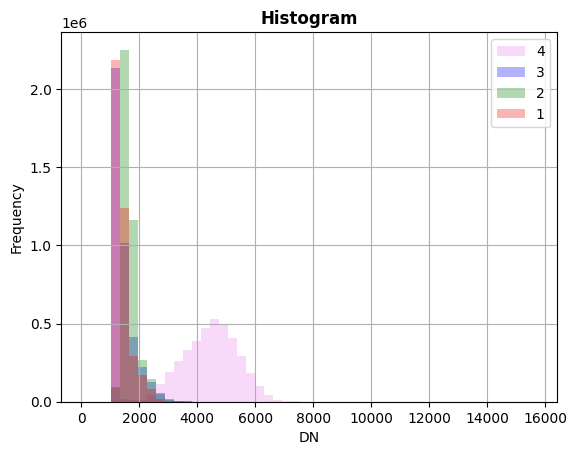
\includegraphics[width=5.5in,height=4.52083in]{02-RehaussementVisualisationImages_files/figure-html/cell-8-output-1.png}
\caption{}
\end{figure}

Pour l'affichage des images, la fonction \texttt{imshow} permet
d'afficher une matrice 2D à une dimension en format float ou une matrice
RVB avec 3 bandes. Il est important que les dimensions de la matrice
soient dans l'ordre hauteur, largeur et bande.

\phantomsection\label{a310105f}
\phantomsection\label{cb7}
\begin{Shaded}
\begin{Highlighting}[]
\ImportTok{import}\NormalTok{ matplotlib.pyplot }\ImportTok{as}\NormalTok{ plt}
\NormalTok{fig, ax}\OperatorTok{=}\NormalTok{ plt.subplots(figsize}\OperatorTok{=}\NormalTok{(}\DecValTok{6}\NormalTok{, }\DecValTok{5}\NormalTok{))}
\NormalTok{plt.imshow(img\_rgbnir[}\DecValTok{0}\NormalTok{].data)}
\NormalTok{plt.show()}
\end{Highlighting}
\end{Shaded}

\begin{figure}
\centering
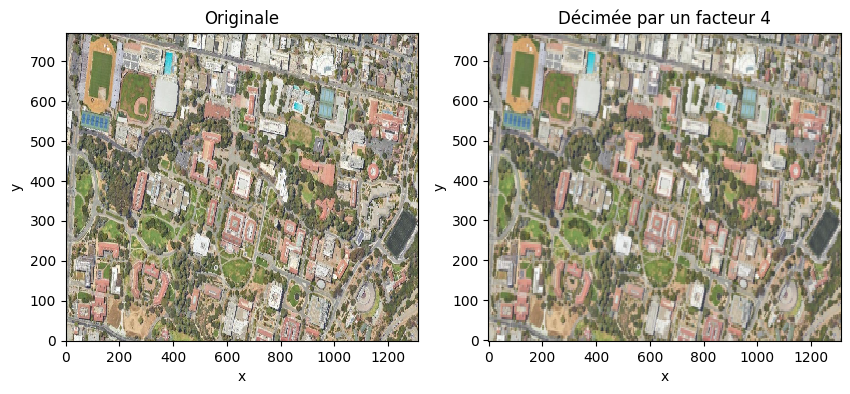
\includegraphics[width=5.03125in,height=4.52083in]{02-RehaussementVisualisationImages_files/figure-html/cell-9-output-1.png}
\caption{}
\end{figure}

Pour un affichage à 3 bandes, les valeurs seront clippées entre 0 et 1,
il est donc nécessaire de normaliser les valeurs avant l'affichage:

\phantomsection\label{f07a293b}
\phantomsection\label{cb8}
\begin{Shaded}
\begin{Highlighting}[]
\ImportTok{import}\NormalTok{ matplotlib.pyplot }\ImportTok{as}\NormalTok{ plt}
\NormalTok{fig, ax}\OperatorTok{=}\NormalTok{ plt.subplots(figsize}\OperatorTok{=}\NormalTok{(}\DecValTok{6}\NormalTok{, }\DecValTok{5}\NormalTok{))}
\NormalTok{plt.imshow(img\_rgbnir.data.transpose(}\DecValTok{1}\NormalTok{,}\DecValTok{2}\NormalTok{,}\DecValTok{0}\NormalTok{)}\OperatorTok{/}\FloatTok{2500.0}\NormalTok{)}
\NormalTok{plt.show()}
\end{Highlighting}
\end{Shaded}

\begin{figure}
\centering
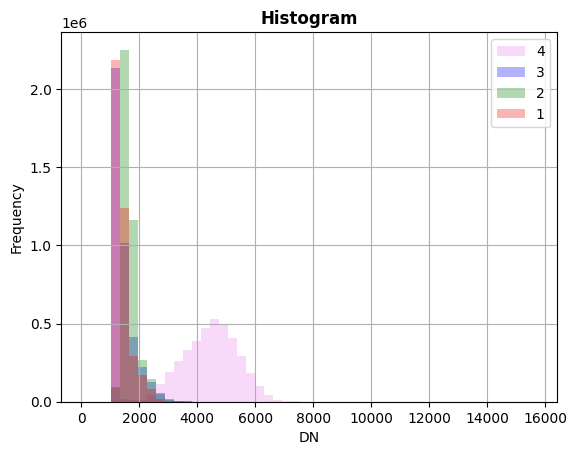
\includegraphics[width=5.03125in,height=4.52083in]{02-RehaussementVisualisationImages_files/figure-html/cell-10-output-1.png}
\caption{}
\end{figure}

On remarquera les valeurs des axes \texttt{x} et \texttt{y} avec une
origine en haut à gauche. Ceci est un référentiel purement matricielle
(lignes et colonnes), il n'y a pas de géoréférence ici. Pour pallier à
cette limitation, les librairies \texttt{rasterio} et \texttt{xarray}
proposent une extension de la fonction \texttt{imshow} permettant
d'afficher les coordonnées cartographiques ainsi qu'un contrôle la
dynamique de l'image:

\phantomsection\label{c9cfdfff}
\phantomsection\label{cb9}
\begin{Shaded}
\begin{Highlighting}[]
\ImportTok{import}\NormalTok{ rioxarray }\ImportTok{as}\NormalTok{ rxr}
\NormalTok{fig, ax}\OperatorTok{=}\NormalTok{ plt.subplots(figsize}\OperatorTok{=}\NormalTok{(}\DecValTok{6}\NormalTok{, }\DecValTok{5}\NormalTok{))}
\NormalTok{img\_rgbnir.sel(band}\OperatorTok{=}\NormalTok{[}\DecValTok{1}\NormalTok{,}\DecValTok{2}\NormalTok{,}\DecValTok{3}\NormalTok{]).plot.imshow(vmin}\OperatorTok{=}\DecValTok{86}\NormalTok{, vmax}\OperatorTok{=}\DecValTok{5000}\NormalTok{)}
\NormalTok{ax.set\_title(}\StringTok{\textquotesingle{}Imshow avec rioxarray\textquotesingle{}}\NormalTok{)}
\NormalTok{plt.show()}
\end{Highlighting}
\end{Shaded}

\begin{figure}
\centering
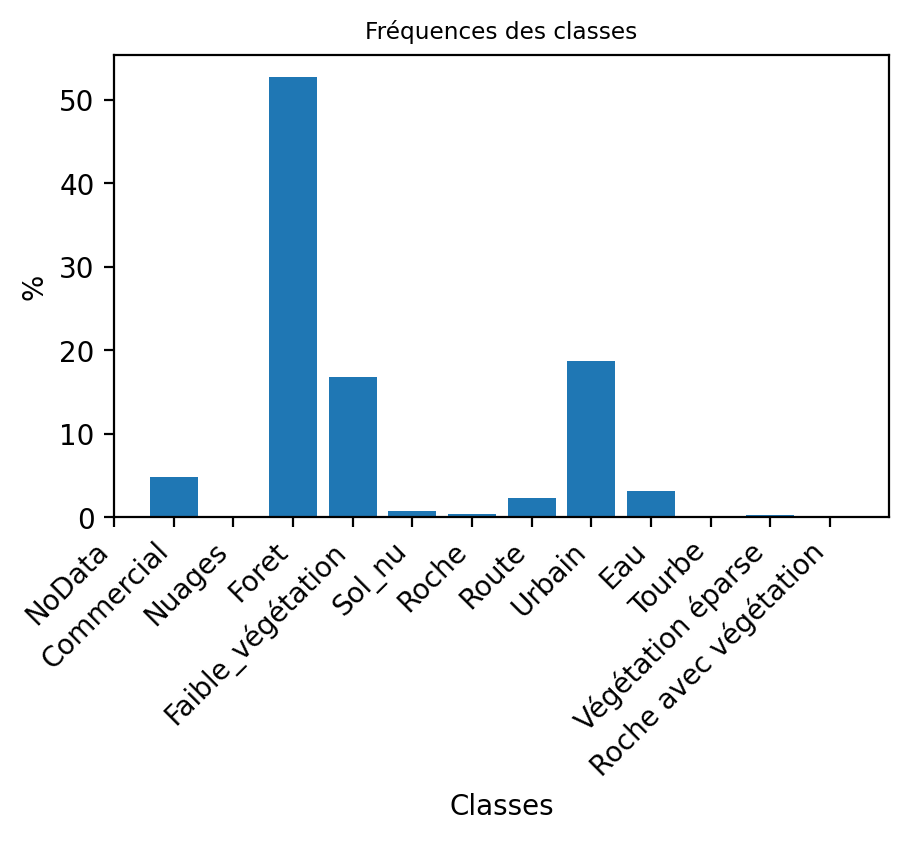
\includegraphics[width=6.13542in,height=4.875in]{02-RehaussementVisualisationImages_files/figure-html/cell-11-output-1.png}
\caption{}
\end{figure}

\subsection{\texorpdfstring{{3.3} Réhaussements
visuels}{3.3 Réhaussements visuels}}\label{ruxe9haussements-visuels}

Le but du réhaussement visuel d'une image vise principalement à
améliorer la qualité visuelle d'une image en améliorant le contraste, la
dynamique ou la texture d'une image. De manière générale, ce
réhaussement ne modifie pas la donnée d'origine mais est plutôt
appliquée dynamiquement à l'affichage pour des fins d'inspection
visuelle.

\subsubsection{\texorpdfstring{{3.3.1} Statistiques d'une
image}{3.3.1 Statistiques d'une image}}\label{statistiques-dune-image}

On peut considérer un ensemble de statistique globales pour chacune des
bandes d'une image: - valeurs minimales et maximales - valeurs moyennes,
médianes et quantiles - écart-types, skewness et kurtosis Ces
statistiques doivent être calculées pour chaque bande d'une image
multispectrale.

En ligne de commande, \texttt{gdalinfo} permet d'interroger rapidement
un fichier image pour connaitre les statistiques de base:

\phantomsection\label{39268283}
\phantomsection\label{cb10}
\begin{Shaded}
\begin{Highlighting}[]
\OperatorTok{!}\NormalTok{gdalinfo }\OperatorTok{{-}}\NormalTok{stats landsat7.tif}
\end{Highlighting}
\end{Shaded}

\begin{verbatim}
Driver: GTiff/GeoTIFF
Files: landsat7.tif
       landsat7.tif.aux.xml
Size is 2181, 1917
Coordinate System is:
PROJCS["WGS 84 / Pseudo-Mercator",
    GEOGCS["WGS 84",
        DATUM["WGS_1984",
            SPHEROID["WGS 84",6378137,298.257223563,
                AUTHORITY["EPSG","7030"]],
            AUTHORITY["EPSG","6326"]],
        PRIMEM["Greenwich",0,
            AUTHORITY["EPSG","8901"]],
        UNIT["degree",0.0174532925199433,
            AUTHORITY["EPSG","9122"]],
        AUTHORITY["EPSG","4326"]],
    PROJECTION["Mercator_1SP"],
    PARAMETER["central_meridian",0],
    PARAMETER["scale_factor",1],
    PARAMETER["false_easting",0],
    PARAMETER["false_northing",0],
    UNIT["metre",1,
        AUTHORITY["EPSG","9001"]],
    AXIS["X",EAST],
    AXIS["Y",NORTH],
    EXTENSION["PROJ4","+proj=merc +a=6378137 +b=6378137 +lat_ts=0.0 +lon_0=0.0 +x_0=0.0 +y_0=0 +k=1.0 +units=m +nadgrids=@null +wktext +no_defs"],
    AUTHORITY["EPSG","3857"]]
Origin = (-13651650.000000000000000,4576290.000000000000000)
Pixel Size = (30.000000000000000,-30.000000000000000)
Metadata:
  AREA_OR_POINT=Area
  OVR_RESAMPLING_ALG=NEAREST
  TIFFTAG_RESOLUTIONUNIT=1 (unitless)
  TIFFTAG_XRESOLUTION=1
  TIFFTAG_YRESOLUTION=1
Image Structure Metadata:
  COMPRESSION=DEFLATE
  INTERLEAVE=PIXEL
Corner Coordinates:
Upper Left  (-13651650.000, 4576290.000) (122d38' 5.49"W, 37d58'40.08"N)
Lower Left  (-13651650.000, 4518780.000) (122d38' 5.49"W, 37d34'10.00"N)
Upper Right (-13586220.000, 4576290.000) (122d 2'49.53"W, 37d58'40.08"N)
Lower Right (-13586220.000, 4518780.000) (122d 2'49.53"W, 37d34'10.00"N)
Center      (-13618935.000, 4547535.000) (122d20'27.51"W, 37d46'26.05"N)
Band 1 Block=512x512 Type=Byte, ColorInterp=Red
  Min=19.000 Max=233.000 
  Minimum=19.000, Maximum=233.000, Mean=98.433, StdDev=21.164
  NoData Value=0
  Overviews: 1091x959, 546x480
  Metadata:
    STATISTICS_MAXIMUM=233
    STATISTICS_MEAN=98.433096940153
    STATISTICS_MINIMUM=19
    STATISTICS_STDDEV=21.164021026458
Band 2 Block=512x512 Type=Byte, ColorInterp=Green
  Min=19.000 Max=178.000 
  Minimum=19.000, Maximum=178.000, Mean=55.068, StdDev=22.204
  NoData Value=0
  Overviews: 1091x959, 546x480
  Metadata:
    STATISTICS_MAXIMUM=178
    STATISTICS_MEAN=55.067787534804
    STATISTICS_MINIMUM=19
    STATISTICS_STDDEV=22.203571974581
Band 3 Block=512x512 Type=Byte, ColorInterp=Blue
  Min=19.000 Max=187.000 
  Minimum=19.000, Maximum=187.000, Mean=43.341, StdDev=20.330
  NoData Value=0
  Overviews: 1091x959, 546x480
  Metadata:
    STATISTICS_MAXIMUM=187
    STATISTICS_MEAN=43.340507443056
    STATISTICS_MINIMUM=19
    STATISTICS_STDDEV=20.32987736339
\end{verbatim}

Les librairies de base comme \texttt{xarray} et \texttt{numpy} peuvent
facilement produire des statistiques comme avec la fonction
\href{https://rasterio.readthedocs.io/en/stable/api/rasterio.io.html\#rasterio.io.BufferedDatasetWriter.stats}{stats}:

\phantomsection\label{f1e49069}
\phantomsection\label{cb12}
\begin{Shaded}
\begin{Highlighting}[]
\ImportTok{import}\NormalTok{ rasterio }\ImportTok{as}\NormalTok{ rio}
\ImportTok{import}\NormalTok{ numpy }\ImportTok{as}\NormalTok{ np}
\ControlFlowTok{with}\NormalTok{ rio.}\BuiltInTok{open}\NormalTok{(}\StringTok{\textquotesingle{}landsat7.tif\textquotesingle{}}\NormalTok{) }\ImportTok{as}\NormalTok{ src:}
\NormalTok{    stats}\OperatorTok{=}\NormalTok{ src.stats()}
    \BuiltInTok{print}\NormalTok{(stats)}
\end{Highlighting}
\end{Shaded}

La librairie \texttt{xarray} donne accès à des fonctionnalités plus
sophistiquées comme le calcul des quantiles:

\phantomsection\label{57eddff8}
\phantomsection\label{cb13}
\begin{Shaded}
\begin{Highlighting}[]
\ImportTok{import}\NormalTok{ rioxarray }\ImportTok{as}\NormalTok{ riox}
\ControlFlowTok{with}\NormalTok{ riox.open\_rasterio(}\StringTok{\textquotesingle{}landsat7.tif\textquotesingle{}}\NormalTok{, masked}\OperatorTok{=} \VariableTok{True}\NormalTok{) }\ImportTok{as}\NormalTok{ src:}
    \BuiltInTok{print}\NormalTok{(src)}
\NormalTok{quantiles }\OperatorTok{=}\NormalTok{ src.quantile(dim}\OperatorTok{=}\NormalTok{[}\StringTok{\textquotesingle{}x\textquotesingle{}}\NormalTok{,}\StringTok{\textquotesingle{}y\textquotesingle{}}\NormalTok{], q}\OperatorTok{=}\NormalTok{[}\FloatTok{.025}\NormalTok{,}\FloatTok{.25}\NormalTok{,}\FloatTok{.5}\NormalTok{,}\FloatTok{.75}\NormalTok{,}\FloatTok{.975}\NormalTok{])}
\NormalTok{quantiles}
\end{Highlighting}
\end{Shaded}

\begin{verbatim}
<xarray.DataArray (band: 3, y: 1917, x: 2181)> Size: 50MB
[12542931 values with dtype=float32]
Coordinates:
  * band         (band) int64 24B 1 2 3
  * x            (x) float64 17kB -1.365e+07 -1.365e+07 ... -1.359e+07
  * y            (y) float64 15kB 4.576e+06 4.576e+06 ... 4.519e+06 4.519e+06
    spatial_ref  int64 8B 0
Attributes:
    AREA_OR_POINT:           Area
    OVR_RESAMPLING_ALG:      NEAREST
    TIFFTAG_RESOLUTIONUNIT:  1 (unitless)
    TIFFTAG_XRESOLUTION:     1
    TIFFTAG_YRESOLUTION:     1
    STATISTICS_MAXIMUM:      233
    STATISTICS_MEAN:         98.433096940153
    STATISTICS_MINIMUM:      19
    STATISTICS_STDDEV:       21.164021026458
    scale_factor:            1.0
    add_offset:              0.0
\end{verbatim}

\begin{Shaded}
\begin{Highlighting}[]
\NormalTok{\textless{}xarray.DataArray (quantile: 5, band: 3)\textgreater{} Size: 120B}
\NormalTok{array([[ 54.,  19.,  19.],}
\NormalTok{       [ 85.,  38.,  27.],}
\NormalTok{       [ 99.,  54.,  38.],}
\NormalTok{       [111.,  69.,  57.],}
\NormalTok{       [140., 102.,  89.]])}
\NormalTok{Coordinates:}
\NormalTok{  * band      (band) int64 24B 1 2 3}
\NormalTok{  * quantile  (quantile) float64 40B 0.025 0.25 0.5 0.75 0.975}
\end{Highlighting}
\end{Shaded}

xarray.DataArray

\begin{itemize}
\tightlist
\item
  {quantile}: 5
\item
  {band}: 3
\end{itemize}

{54.0 19.0 19.0 85.0 38.0 27.0 ... 111.0 69.0 57.0 140.0 102.0 89.0}

\begin{verbatim}
array([[ 54.,  19.,  19.],
       [ 85.,  38.,  27.],
       [ 99.,  54.,  38.],
       [111.,  69.,  57.],
       [140., 102.,  89.]])
\end{verbatim}

Coordinates: {(2)}

{band}

(band)

int64

1 2 3

\begin{verbatim}
array([1, 2, 3])
\end{verbatim}

{quantile}

(quantile)

float64

0.025 0.25 0.5 0.75 0.975

\begin{verbatim}
array([0.025, 0.25 , 0.5  , 0.75 , 0.975])
\end{verbatim}

Indexes: {(2)}

band

PandasIndex

\begin{verbatim}
PandasIndex(Index([1, 2, 3], dtype='int64', name='band'))
\end{verbatim}

quantile

PandasIndex

\begin{verbatim}
PandasIndex(Index([0.025, 0.25, 0.5, 0.75, 0.975], dtype='float64', name='quantile'))
\end{verbatim}

Attributes: {(0)}

\paragraph{\texorpdfstring{{3.3.1.1} Calcul de
l'histogramme}{3.3.1.1 Calcul de l'histogramme}}\label{calcul-de-lhistogramme}

Le calcul d'un histogramme pour une image (une bande) permet d'avoir une
vue plus détaillée de la répartition des valeurs radiométriques. Le
calcul d'un histogramme nécessite minimalement de faire le choix d'une
valeur du nombre de \emph{bins} (ou de la largeur). Un \emph{bin} est un
intervalle de valeurs pour lequel on peut calculer le nombre de valeurs
observées dans l'image. La fonction de base pour ce type de calcul est
la fonction \texttt{numpy.histogram()}:

\phantomsection\label{cc15c57f}
\phantomsection\label{cb15}
\begin{Shaded}
\begin{Highlighting}[]
\ImportTok{import}\NormalTok{ numpy }\ImportTok{as}\NormalTok{ np}
\NormalTok{array }\OperatorTok{=}\NormalTok{ np.random.randint(}\DecValTok{0}\NormalTok{,}\DecValTok{10}\NormalTok{,}\DecValTok{100}\NormalTok{) }\CommentTok{\# 100 valeurs aléatoires entre 0 et 10}
\NormalTok{hist, bin\_limites }\OperatorTok{=}\NormalTok{ np.histogram(array, density}\OperatorTok{=}\VariableTok{True}\NormalTok{)}
\BuiltInTok{print}\NormalTok{(}\StringTok{\textquotesingle{}valeurs :\textquotesingle{}}\NormalTok{,hist)}
\BuiltInTok{print}\NormalTok{(}\StringTok{\textquotesingle{};imites :\textquotesingle{}}\NormalTok{,bin\_limites)}
\end{Highlighting}
\end{Shaded}

\begin{verbatim}
valeurs : [0.11111111 0.11111111 0.12222222 0.12222222 0.11111111 0.08888889
 0.13333333 0.06666667 0.12222222 0.12222222]
;imites : [0.  0.9 1.8 2.7 3.6 4.5 5.4 6.3 7.2 8.1 9. ]
\end{verbatim}

Le calcul se fait avec 10 intervalles par défaut.

\phantomsection\label{deb9e2ed}
\phantomsection\label{cb17}
\begin{Shaded}
\begin{Highlighting}[]
\NormalTok{plt.bar(bin\_limites[:}\OperatorTok{{-}}\DecValTok{1}\NormalTok{],hist)}
\NormalTok{plt.show()}
\end{Highlighting}
\end{Shaded}

\begin{figure}
\centering
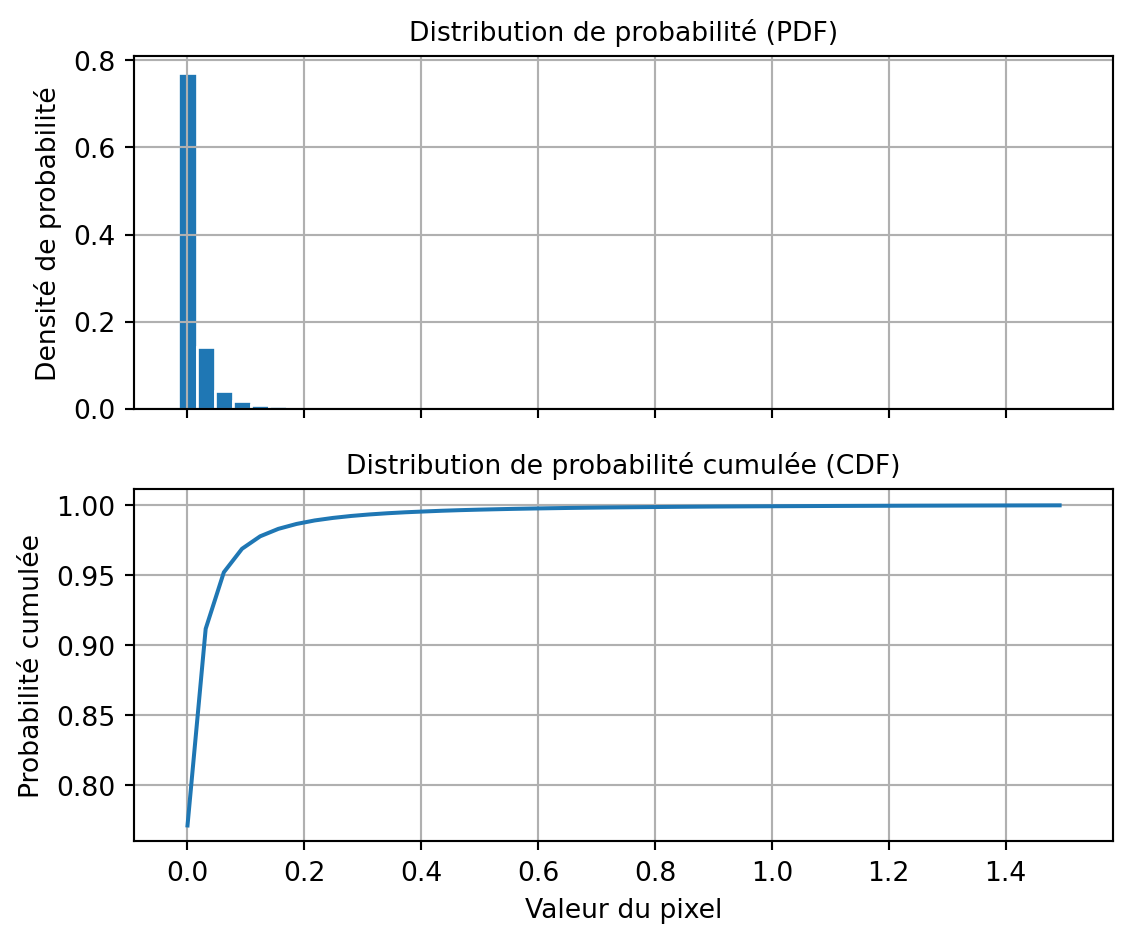
\includegraphics[width=7.09375in,height=4.52083in]{02-RehaussementVisualisationImages_files/figure-html/cell-16-output-1.png}
\caption{}
\end{figure}

Pour des besoins de visualisation, le calcul des valeurs extrêmes de
l'histogramme peut aussi se faire via les quantiles comme discutés
auparavant.

\subparagraph{\texorpdfstring{{3.3.1.1.1} Visualisation des
histogrammes}{3.3.1.1.1 Visualisation des histogrammes}}\label{visualisation-des-histogrammes}

La librarie \texttt{rasterio} est probablement l'outil le plus simples
pour visualiser rapidement des histogrammes sur une image
multi-spectrale:

\phantomsection\label{e670a4b6}
\phantomsection\label{cb18}
\begin{Shaded}
\begin{Highlighting}[]
\ImportTok{import}\NormalTok{ rasterio }\ImportTok{as}\NormalTok{ rio}
\ImportTok{from}\NormalTok{ rasterio.plot }\ImportTok{import}\NormalTok{ show\_hist}
\ControlFlowTok{with}\NormalTok{ rio.}\BuiltInTok{open}\NormalTok{(}\StringTok{\textquotesingle{}RGBNIR\_of\_S2A.tif\textquotesingle{}}\NormalTok{) }\ImportTok{as}\NormalTok{ src:}
\NormalTok{  show\_hist(src, bins}\OperatorTok{=}\DecValTok{50}\NormalTok{, lw}\OperatorTok{=}\FloatTok{0.0}\NormalTok{, stacked}\OperatorTok{=}\VariableTok{False}\NormalTok{, alpha}\OperatorTok{=}\FloatTok{0.3}\NormalTok{,histtype}\OperatorTok{=}\StringTok{\textquotesingle{}stepfilled\textquotesingle{}}\NormalTok{, title}\OperatorTok{=}\StringTok{"Histogram"}\NormalTok{)}
\end{Highlighting}
\end{Shaded}

\begin{figure}
\centering
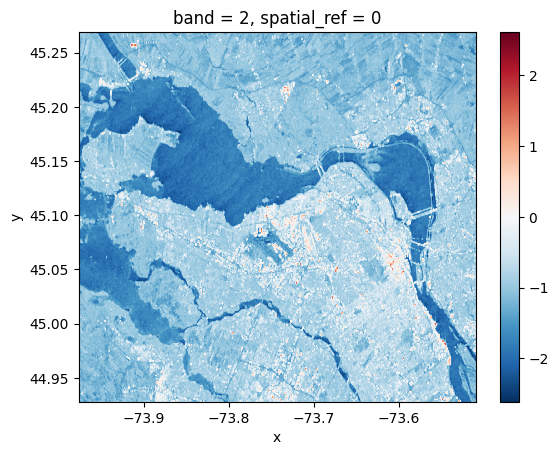
\includegraphics[width=7.27083in,height=4.875in]{02-RehaussementVisualisationImages_files/figure-html/cell-17-output-1.png}
\caption{}
\end{figure}

\subsubsection{\texorpdfstring{{3.3.2} Réhaussements
linéaires}{3.3.2 Réhaussements linéaires}}\label{ruxe9haussements-linuxe9aires}

Le réhaussement linéaire (\emph{linear stretch}) d'une image est la
forme la plus simple de réhaussement, elle consiste 1) à optimiser les
valeurs des pixels d'une image afin de maximiser la dynamique
disponibles à l'affichage, ou 2) changer le format de stockage des
valeurs (e.g.~de 8 bit à 16 bit):

\phantomsection\label{eq-rehauss-lin}{{\textbackslash{[}
\textbackslash text\{nouvelle valeur d\textquotesingle un pixel\} =
\textbackslash frac\{\textbackslash text\{valeur d\textquotesingle un
pixel\} - min\_0\}\{max\_0 - min\_0\}\textbackslash times (max\_1 -
min\_1)+min\_1 \textbackslash tag\{3.1\}\textbackslash{]}}}

Par cette opération, on passe de la dynamique de départ
({\textbackslash(max\_0 - min\_0\textbackslash)}) vers la dynamique
cible ({\textbackslash(max\_1 - min\_1\textbackslash)}). Bien que cette
opération semble triviale, il est important d'être conscient des trois
contraintes suivantes: 1. \textbf{Faire attention à la dynamique cible},
ainsi, pour sauvegarder une image en format 8 bit, on utilisera alors
{\textbackslash(max\_1=255\textbackslash)} et
{\textbackslash(min\_1=0\textbackslash)}. 2. \textbf{Préservation de la
valeur de no data} : il faut faire attention à la valeur
{\textbackslash(min\_1\textbackslash)} dans le cas d'une valeur présente
pour \emph{no\_data}. Par exemple, si \emph{no\_data=0} alors il faut
s'assurer que {\textbackslash(min\_1\textgreater0\textbackslash)}. 3.
\textbf{Précision du calcul} : si possible réaliser la division
ci-dessus en format \emph{float}

\paragraph{\texorpdfstring{{3.3.2.1} Cas des histogrammes
asymétriques}{3.3.2.1 Cas des histogrammes asymétriques}}\label{cas-des-histogrammes-asymuxe9triques}

Dans certains cas, la distribution de valeurs est très asymétrique et
présente une longue queue avec des valeurs extrêmes élevées. Le cas des
images SAR est particulièrement représentatif de ce type de données. En
effet, celles-ci peuvent présenter une distribution de valeurs de type
exponentiel. Il est alors préférable d'utiliser des
\href{https://fr.wikipedia.org/wiki/Centile}{percentiles} au préalable
afin d'explorer la forme de l'histogramme et la distribution des
valeurs:

\phantomsection\label{34d21d70}
\phantomsection\label{cb19}
\begin{Shaded}
\begin{Highlighting}[]
\NormalTok{NO\_DATA\_FLOAT}\OperatorTok{=} \OperatorTok{{-}}\FloatTok{999.0}
\CommentTok{\# on prend tous les pixels de la première bande}
\NormalTok{values }\OperatorTok{=}\NormalTok{ img\_SAR[}\DecValTok{0}\NormalTok{].values.flatten().astype(}\BuiltInTok{float}\NormalTok{)}
\CommentTok{\# on exclut les valeurs invalides}
\NormalTok{values }\OperatorTok{=}\NormalTok{ values[}\OperatorTok{\textasciitilde{}}\NormalTok{np.isnan(values)]}
\CommentTok{\# on exclut le no data}
\NormalTok{values }\OperatorTok{=}\NormalTok{ values[values}\OperatorTok{!=}\NormalTok{NO\_DATA\_FLOAT]}
\CommentTok{\# calcul des percentiles}
\NormalTok{percentiles\_position}\OperatorTok{=}\NormalTok{ (}\DecValTok{0}\NormalTok{,}\FloatTok{0.1}\NormalTok{,}\DecValTok{1}\NormalTok{,}\DecValTok{2}\NormalTok{,}\DecValTok{50}\NormalTok{,}\DecValTok{98}\NormalTok{,}\DecValTok{99}\NormalTok{,}\FloatTok{99.9}\NormalTok{,}\DecValTok{100}\NormalTok{)}
\NormalTok{percentiles}\OperatorTok{=} \BuiltInTok{dict}\NormalTok{(}\BuiltInTok{zip}\NormalTok{(percentiles\_position, np.percentile(values, percentiles\_position)))}
\BuiltInTok{print}\NormalTok{(percentiles)}
\end{Highlighting}
\end{Shaded}

\begin{verbatim}
{0: np.float64(8.172580237442162e-06), 0.1: np.float64(1.588739885482937e-05), 1: np.float64(8.657756850880105e-05), 2: np.float64(0.00018846066552214325), 50: np.float64(0.012372820172458887), 98: np.float64(0.1719470709562302), 99: np.float64(0.27963151514529694), 99.9: np.float64(1.5235805057287233), 100: np.float64(483.223876953125)}
\end{verbatim}

La première observation que l'on peut faire est que la valeur médiane
(\texttt{0.012}) est très faible, 50\% des valeurs sont inférieures
cette valeur alors que valeur maximale (\texttt{483}) est 10,000 fois
plus élevée! Une façon de visualiser cette distribution de valeurs est
d'utiliser
\href{https://matplotlib.org/stable/api/_as_gen/matplotlib.pyplot.boxplot.html}{\texttt{boxplot}}
et
\href{https://matplotlib.org/stable/api/_as_gen/matplotlib.pyplot.violinplot.html}{\texttt{violinplot}}
de la librairie \texttt{matplotlib}:

\phantomsection\label{d95a1929}
\phantomsection\label{cb21}
\begin{Shaded}
\begin{Highlighting}[]
\NormalTok{fig, ax }\OperatorTok{=}\NormalTok{ plt.subplots(nrows}\OperatorTok{=}\DecValTok{2}\NormalTok{, ncols}\OperatorTok{=}\DecValTok{1}\NormalTok{, figsize}\OperatorTok{=}\NormalTok{(}\DecValTok{6}\NormalTok{, }\DecValTok{4}\NormalTok{), sharex}\OperatorTok{=}\VariableTok{True}\NormalTok{)}
\NormalTok{ax[}\DecValTok{0}\NormalTok{].set\_title(}\StringTok{\textquotesingle{}Distribution de la bande 0 de img\_SAR\textquotesingle{}}\NormalTok{, fontsize}\OperatorTok{=}\StringTok{\textquotesingle{}small\textquotesingle{}}\NormalTok{)}
\NormalTok{ax[}\DecValTok{0}\NormalTok{].grid(}\VariableTok{True}\NormalTok{)}
\NormalTok{ax[}\DecValTok{0}\NormalTok{].violinplot(values, orientation  }\OperatorTok{=}\StringTok{\textquotesingle{}horizontal\textquotesingle{}}\NormalTok{, }
\NormalTok{                 quantiles }\OperatorTok{=}\NormalTok{(}\FloatTok{0.01}\NormalTok{,}\FloatTok{0.02}\NormalTok{,}\FloatTok{0.50}\NormalTok{,}\FloatTok{0.98}\NormalTok{,}\FloatTok{0.99}\NormalTok{),}
\NormalTok{                  showmeans}\OperatorTok{=}\VariableTok{False}\NormalTok{,}
\NormalTok{                  showmedians}\OperatorTok{=}\VariableTok{True}\NormalTok{)}
\NormalTok{ax[}\DecValTok{1}\NormalTok{].set\_xlabel(}\StringTok{\textquotesingle{}Valeur des pixels\textquotesingle{}}\NormalTok{)}
\NormalTok{ax[}\DecValTok{1}\NormalTok{].grid(}\VariableTok{True}\NormalTok{)}
\NormalTok{bplot }\OperatorTok{=}\NormalTok{ ax[}\DecValTok{1}\NormalTok{].boxplot(values, notch }\OperatorTok{=} \VariableTok{True}\NormalTok{, orientation  }\OperatorTok{=}\StringTok{\textquotesingle{}horizontal\textquotesingle{}}\NormalTok{)}
\NormalTok{plt.tight\_layout()}
\NormalTok{plt.show()}
\end{Highlighting}
\end{Shaded}

\begin{figure}
\centering
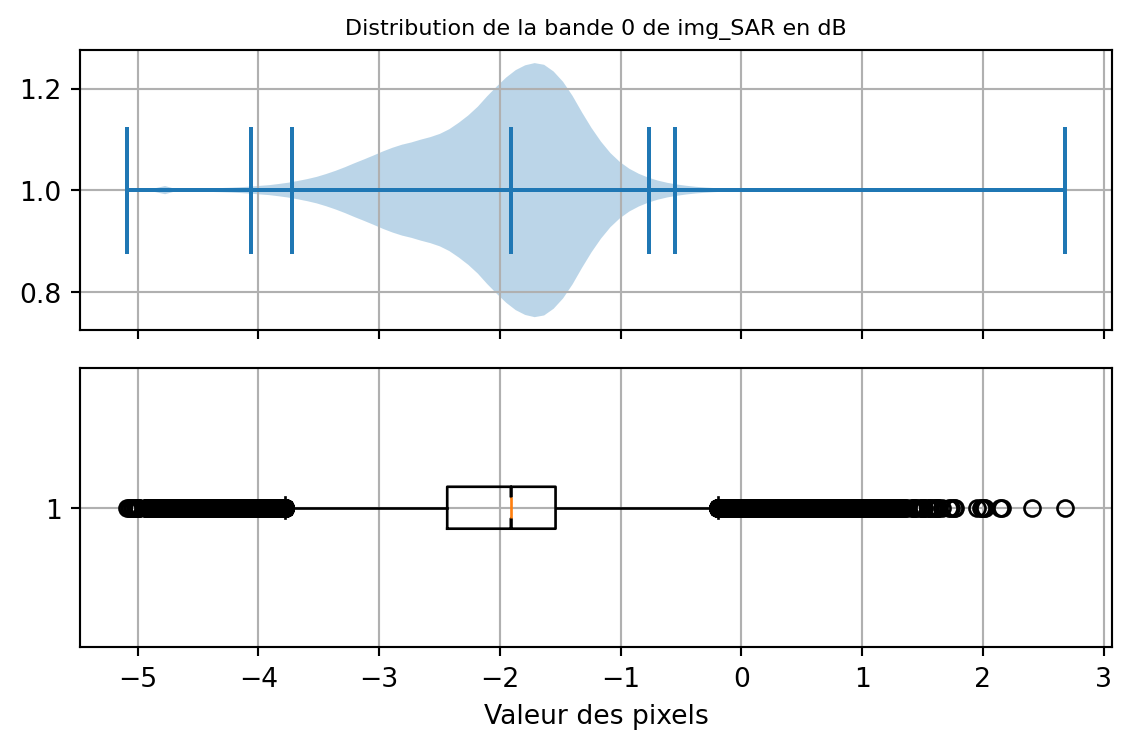
\includegraphics[width=6.13542in,height=4.05208in]{02-RehaussementVisualisationImages_files/figure-html/cell-19-output-1.png}
\caption{}
\end{figure}

Afin de visualiser correctement l'histogramme, il faut se limiter à un
interval de valeurs plus petit. Dans le code ci-dessous, on impose à la
fonction histogramme de compter les valeurs de pixels dans des
intervalles de valeurs fixés par la fonction
\texttt{np.linspace(percentiles{[}0.1{]},percentiles{[}99.9{]},\ 50)} où
\texttt{percentiles{[}0.1{]}} et \texttt{percentiles{[}99.9{]}} sont les
{\textbackslash(0.1\textbackslash\%\textbackslash)} et
{\textbackslash(99.9\textbackslash\%\textbackslash)} percentiles
respectivement:

\phantomsection\label{ec419390}
\phantomsection\label{cb22}
\begin{Shaded}
\begin{Highlighting}[]
\NormalTok{hist, bin\_edges }\OperatorTok{=}\NormalTok{ np.histogram(values, }
\NormalTok{                                bins}\OperatorTok{=}\NormalTok{np.linspace(percentiles[}\FloatTok{0.1}\NormalTok{], }
\NormalTok{                                percentiles[}\FloatTok{99.9}\NormalTok{], }\DecValTok{50}\NormalTok{), }
\NormalTok{                                density}\OperatorTok{=}\VariableTok{True}\NormalTok{)}

\NormalTok{fig, ax }\OperatorTok{=}\NormalTok{ plt.subplots(nrows}\OperatorTok{=}\DecValTok{2}\NormalTok{,ncols}\OperatorTok{=}\DecValTok{1}\NormalTok{,figsize}\OperatorTok{=}\NormalTok{(}\DecValTok{6}\NormalTok{, }\DecValTok{5}\NormalTok{), sharex}\OperatorTok{=}\VariableTok{True}\NormalTok{)}
\NormalTok{ax[}\DecValTok{0}\NormalTok{].bar(bin\_edges[:}\OperatorTok{{-}}\DecValTok{1}\NormalTok{], }
\NormalTok{                hist}\OperatorTok{*}\NormalTok{(bin\_edges[}\DecValTok{1}\NormalTok{]}\OperatorTok{{-}}\NormalTok{bin\_edges[}\DecValTok{0}\NormalTok{]), }
\NormalTok{                width}\OperatorTok{=}\NormalTok{ (bin\_edges[}\DecValTok{1}\NormalTok{]}\OperatorTok{{-}}\NormalTok{bin\_edges[}\DecValTok{0}\NormalTok{]), }
\NormalTok{                edgecolor}\OperatorTok{=} \StringTok{\textquotesingle{}w\textquotesingle{}}\NormalTok{)}
\NormalTok{ax[}\DecValTok{0}\NormalTok{].set\_title(}\StringTok{"Distribution de probabilité (PDF)"}\NormalTok{)}
\NormalTok{ax[}\DecValTok{0}\NormalTok{].set\_ylabel(}\StringTok{"Densité de probabilité"}\NormalTok{)}
\NormalTok{ax[}\DecValTok{0}\NormalTok{].grid(}\VariableTok{True}\NormalTok{)}

\NormalTok{ax[}\DecValTok{1}\NormalTok{].plot(bin\_edges[:}\OperatorTok{{-}}\DecValTok{1}\NormalTok{], }
\NormalTok{            hist.cumsum()}\OperatorTok{*}\NormalTok{(bin\_edges[}\DecValTok{1}\NormalTok{]}\OperatorTok{{-}}\NormalTok{bin\_edges[}\DecValTok{0}\NormalTok{]))}
\NormalTok{ax[}\DecValTok{1}\NormalTok{].set\_title(}\StringTok{"Distribution de probabilité cumulée (CDF)"}\NormalTok{)}
\NormalTok{ax[}\DecValTok{1}\NormalTok{].set\_xlabel(}\StringTok{"Valeur du pixel"}\NormalTok{)}
\NormalTok{ax[}\DecValTok{1}\NormalTok{].set\_ylabel(}\StringTok{"Probabilité cumulée"}\NormalTok{)}
\NormalTok{ax[}\DecValTok{1}\NormalTok{].grid(}\VariableTok{True}\NormalTok{)}
\NormalTok{plt.tight\_layout()}
\NormalTok{plt.show()                              }
\end{Highlighting}
\end{Shaded}

\begin{figure}
\centering
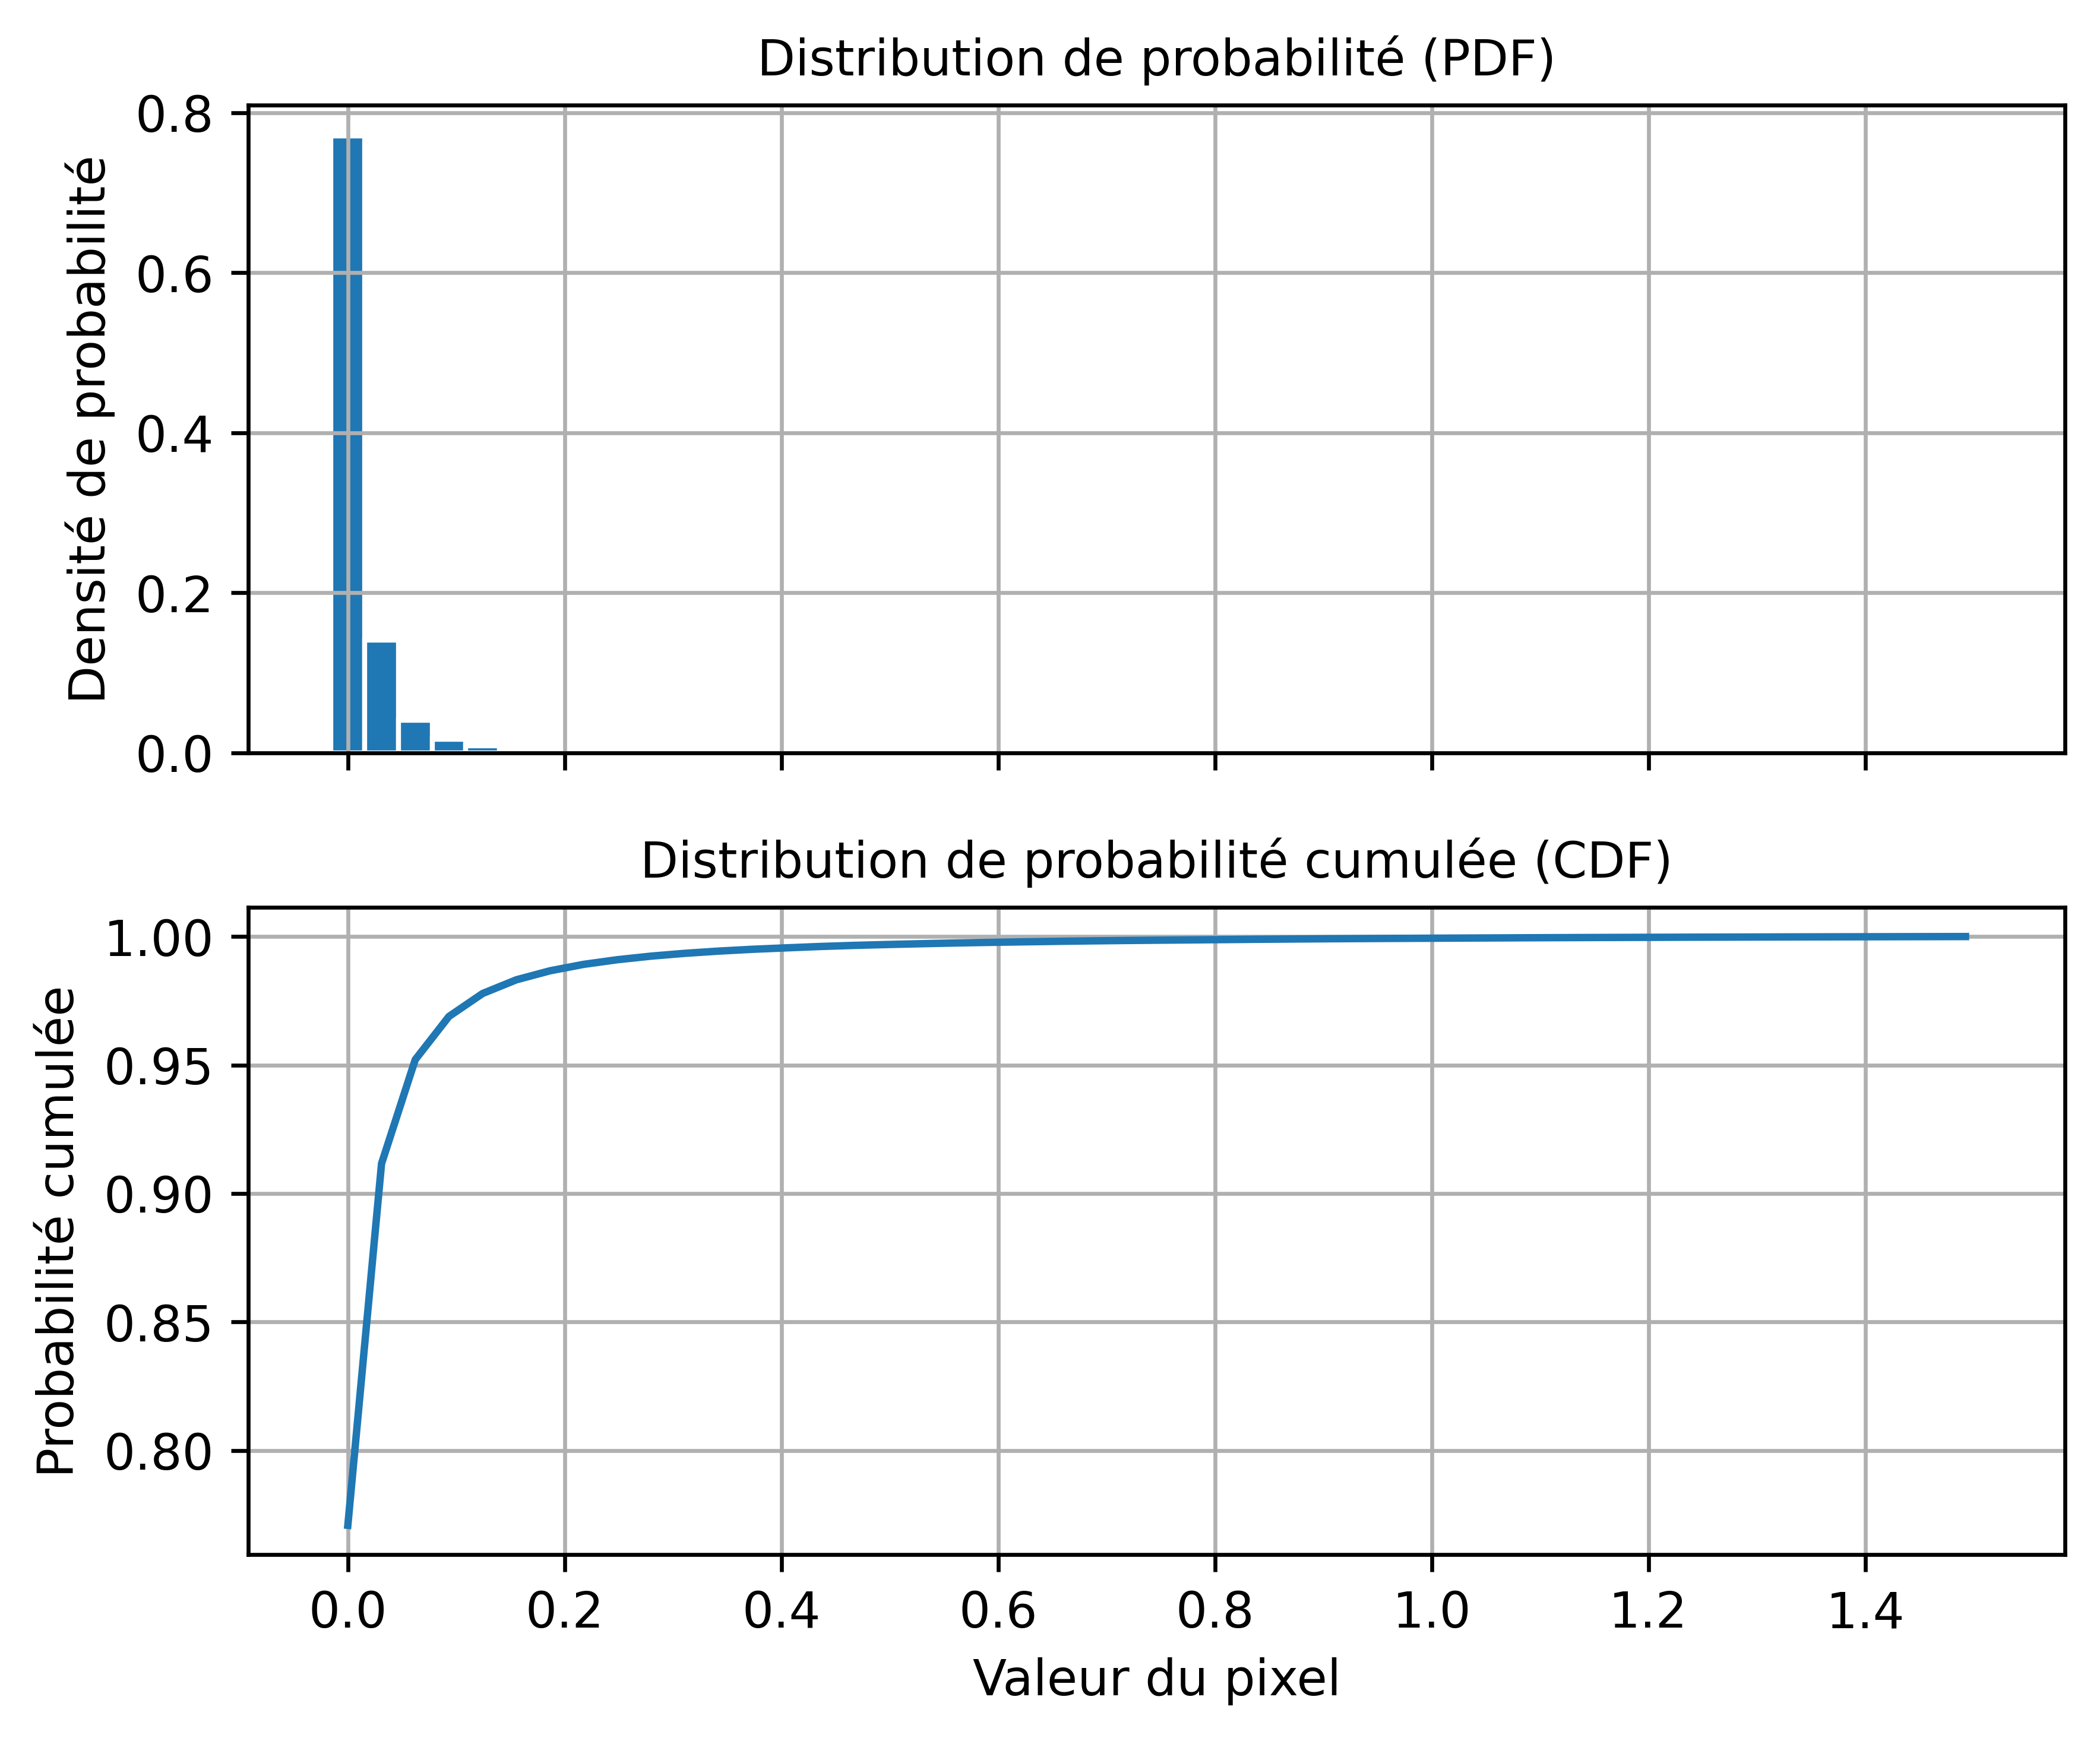
\includegraphics[width=6.14583in,height=5.10417in]{02-RehaussementVisualisationImages_files/figure-html/cell-20-output-1.png}
\caption{}
\end{figure}

Au niveau de l'affichage avec \texttt{matplotlib}, la dynamique peut
être contrôlée directement via les paramètres \texttt{vmin} et
\texttt{vmax} comme ceci:

\phantomsection\label{ed0b7578}
\phantomsection\label{cb23}
\begin{Shaded}
\begin{Highlighting}[]
\NormalTok{fig, ax }\OperatorTok{=}\NormalTok{ plt.subplots(nrows}\OperatorTok{=}\DecValTok{2}\NormalTok{, ncols}\OperatorTok{=}\DecValTok{2}\NormalTok{, figsize}\OperatorTok{=}\NormalTok{(}\DecValTok{6}\NormalTok{, }\DecValTok{5}\NormalTok{), sharex}\OperatorTok{=}\VariableTok{True}\NormalTok{, sharey}\OperatorTok{=}\VariableTok{True}\NormalTok{)}
\NormalTok{[a.axis(}\StringTok{\textquotesingle{}off\textquotesingle{}}\NormalTok{) }\ControlFlowTok{for}\NormalTok{ a }\KeywordTok{in}\NormalTok{ ax.flatten()]}
\NormalTok{ax[}\DecValTok{0}\NormalTok{,}\DecValTok{0}\NormalTok{].imshow(img\_SAR[}\DecValTok{0}\NormalTok{].values, vmin}\OperatorTok{=}\NormalTok{percentiles[}\DecValTok{0}\NormalTok{], vmax}\OperatorTok{=}\NormalTok{percentiles[}\DecValTok{100}\NormalTok{])}
\NormalTok{ax[}\DecValTok{0}\NormalTok{,}\DecValTok{0}\NormalTok{].set\_title(}\SpecialStringTok{f"0\% {-} 100\%=}\SpecialCharTok{\{}\NormalTok{percentiles[}\DecValTok{0}\NormalTok{]}\SpecialCharTok{:2.1f\}}\SpecialStringTok{ {-} }\SpecialCharTok{\{}\NormalTok{percentiles[}\DecValTok{100}\NormalTok{]}\SpecialCharTok{:2.1f\}}\SpecialStringTok{"}\NormalTok{)}
\NormalTok{ax[}\DecValTok{0}\NormalTok{,}\DecValTok{1}\NormalTok{].imshow(img\_SAR[}\DecValTok{0}\NormalTok{].values, vmin}\OperatorTok{=}\NormalTok{percentiles[}\FloatTok{0.1}\NormalTok{], vmax}\OperatorTok{=}\NormalTok{percentiles[}\FloatTok{99.9}\NormalTok{]) }
\NormalTok{ax[}\DecValTok{0}\NormalTok{,}\DecValTok{1}\NormalTok{].set\_title(}\SpecialStringTok{f"0.1\% {-} 99.9\%=}\SpecialCharTok{\{}\NormalTok{percentiles[}\FloatTok{0.1}\NormalTok{]}\SpecialCharTok{:2.1f\}}\SpecialStringTok{ {-} }\SpecialCharTok{\{}\NormalTok{percentiles[}\FloatTok{99.9}\NormalTok{]}\SpecialCharTok{:2.1f\}}\SpecialStringTok{"}\NormalTok{)}
\NormalTok{ax[}\DecValTok{1}\NormalTok{,}\DecValTok{0}\NormalTok{].imshow(img\_SAR[}\DecValTok{0}\NormalTok{].values, vmin}\OperatorTok{=}\NormalTok{percentiles[}\DecValTok{1}\NormalTok{], vmax}\OperatorTok{=}\NormalTok{percentiles[}\DecValTok{99}\NormalTok{]) }
\NormalTok{ax[}\DecValTok{1}\NormalTok{,}\DecValTok{0}\NormalTok{].set\_title(}\SpecialStringTok{f"1\% {-} 99\%=}\SpecialCharTok{\{}\NormalTok{percentiles[}\DecValTok{1}\NormalTok{]}\SpecialCharTok{:2.1f\}}\SpecialStringTok{ {-} }\SpecialCharTok{\{}\NormalTok{percentiles[}\DecValTok{99}\NormalTok{]}\SpecialCharTok{:2.1f\}}\SpecialStringTok{"}\NormalTok{)}
\NormalTok{ax[}\DecValTok{1}\NormalTok{,}\DecValTok{1}\NormalTok{].imshow(img\_SAR[}\DecValTok{0}\NormalTok{].values, vmin}\OperatorTok{=}\NormalTok{percentiles[}\DecValTok{2}\NormalTok{], vmax}\OperatorTok{=}\NormalTok{percentiles[}\DecValTok{98}\NormalTok{]) }
\NormalTok{ax[}\DecValTok{1}\NormalTok{,}\DecValTok{1}\NormalTok{].set\_title(}\SpecialStringTok{f"2\% {-} 98\%=}\SpecialCharTok{\{}\NormalTok{percentiles[}\DecValTok{2}\NormalTok{]}\SpecialCharTok{:2.1f\}}\SpecialStringTok{ {-} }\SpecialCharTok{\{}\NormalTok{percentiles[}\DecValTok{98}\NormalTok{]}\SpecialCharTok{:2.1f\}}\SpecialStringTok{"}\NormalTok{)}
\NormalTok{plt.tight\_layout()}
\end{Highlighting}
\end{Shaded}

\begin{figure}
\centering
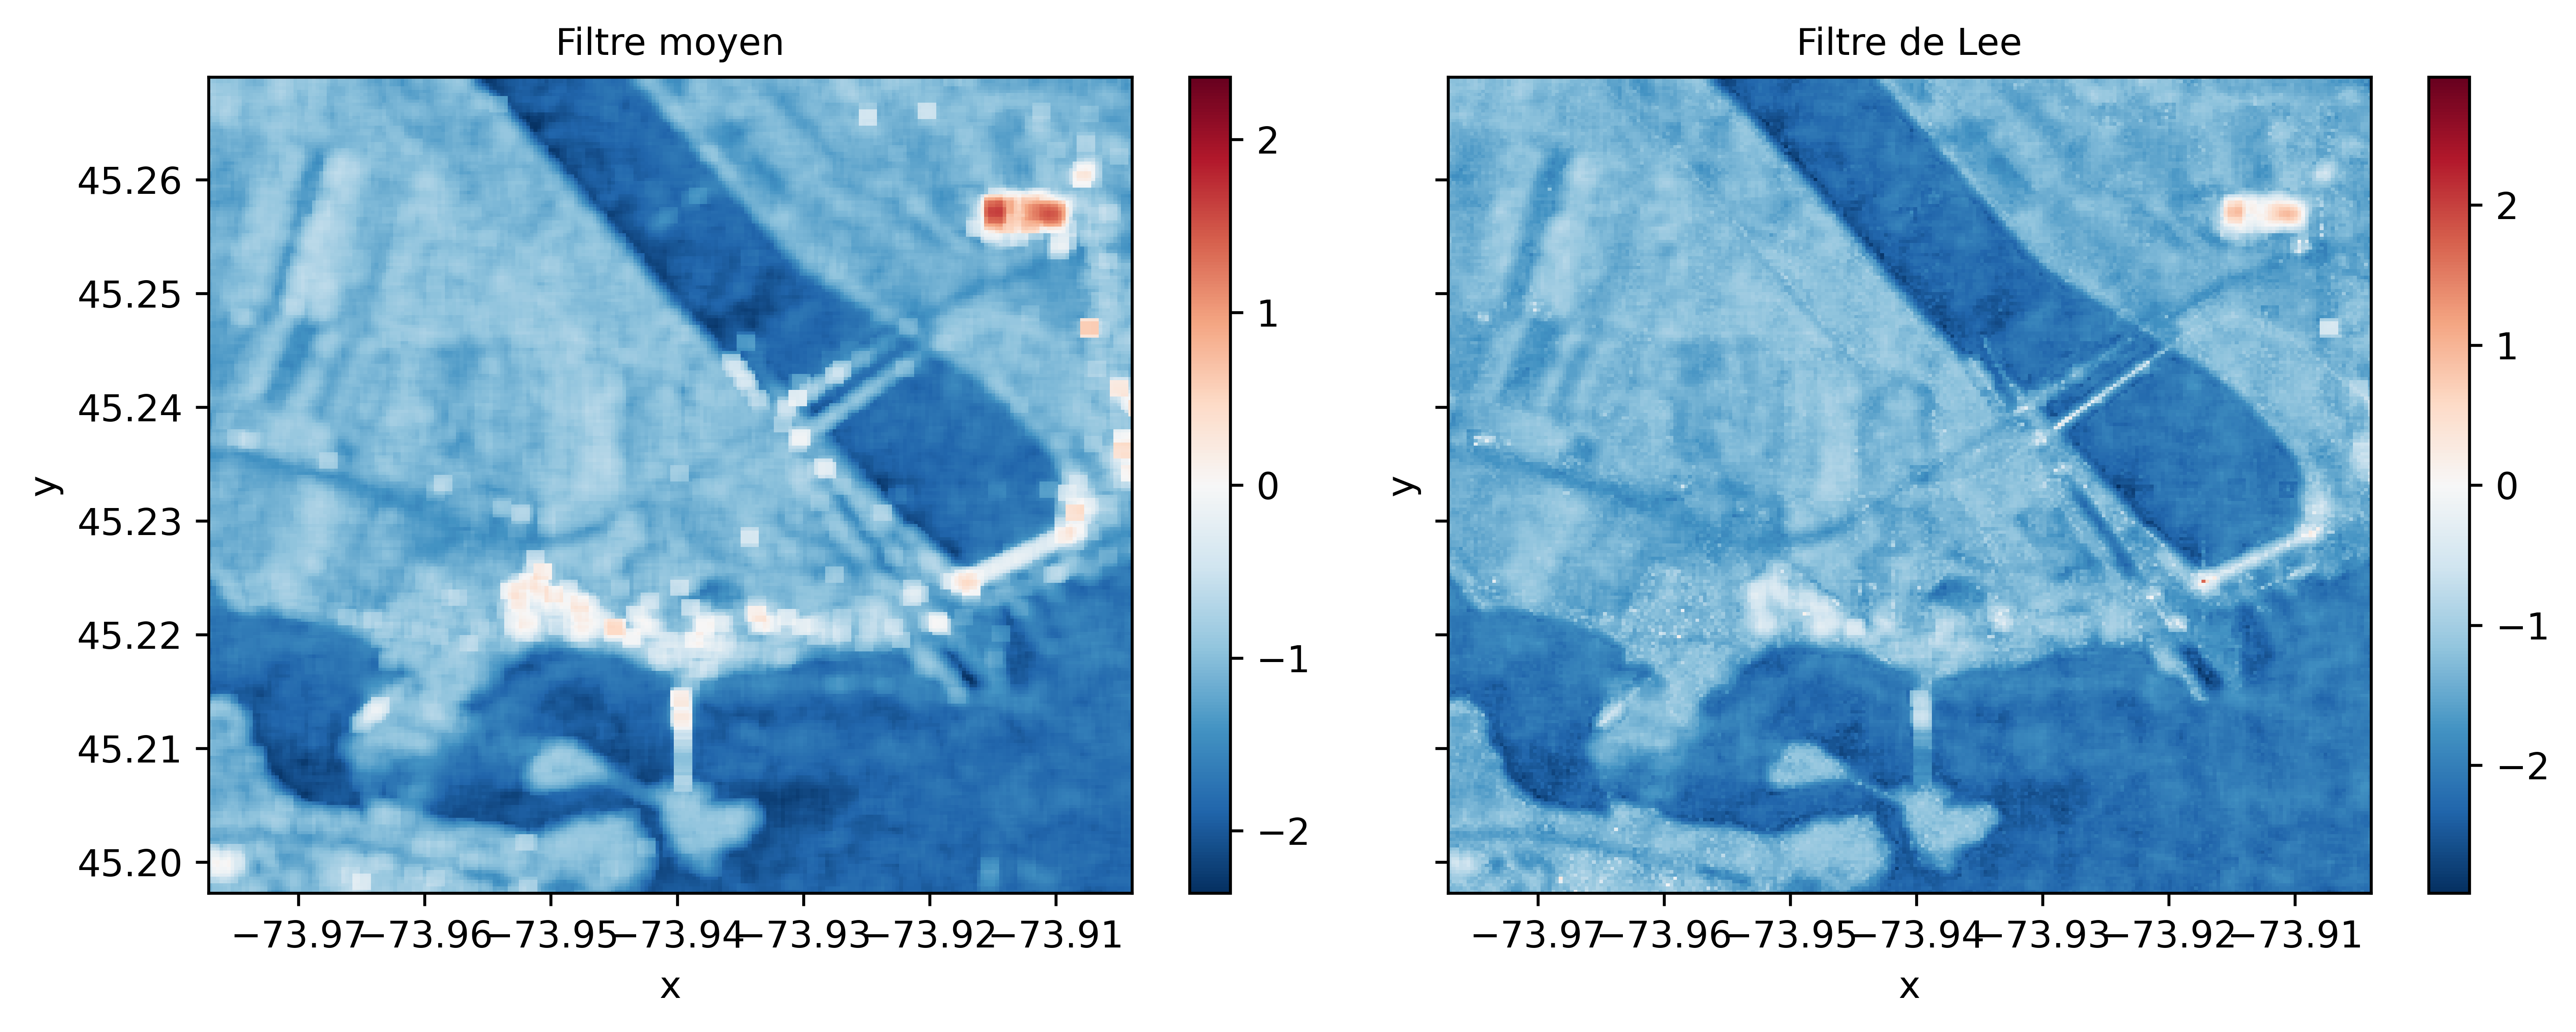
\includegraphics[width=6.14583in,height=5.04167in]{02-RehaussementVisualisationImages_files/figure-html/cell-21-output-1.png}
\caption{}
\end{figure}

\subsubsection{\texorpdfstring{{3.3.3} Réhaussements non
linéaires}{3.3.3 Réhaussements non linéaires}}\label{ruxe9haussements-non-linuxe9aires}

\paragraph{\texorpdfstring{{3.3.3.1} Réhaussement par
fonctions}{3.3.3.1 Réhaussement par fonctions}}\label{ruxe9haussement-par-fonctions}

Le réhaussenent par fonction consiste à appliquer une fonction non
linéaire afin de modifier la dynamique de l'image. Par exemple, pour une
image radar, une transformation populaire est dd'afficher les valeurs de
rétrodiffusion en décibel (\texttt{dB}) via la fonction
\texttt{log10()}.

\phantomsection\label{bfffca0f}
\phantomsection\label{cb24}
\begin{Shaded}
\begin{Highlighting}[]
\NormalTok{percentiles\_position}\OperatorTok{=}\NormalTok{ (}\DecValTok{0}\NormalTok{,}\FloatTok{0.1}\NormalTok{,}\DecValTok{1}\NormalTok{,}\DecValTok{2}\NormalTok{,}\DecValTok{50}\NormalTok{,}\DecValTok{98}\NormalTok{,}\DecValTok{99}\NormalTok{,}\FloatTok{99.9}\NormalTok{,}\DecValTok{100}\NormalTok{)}
\NormalTok{values}\OperatorTok{=}\NormalTok{ np.log10(img\_SAR[}\DecValTok{0}\NormalTok{]).data}
\NormalTok{percentiles\_db}\OperatorTok{=} \BuiltInTok{dict}\NormalTok{(}\BuiltInTok{zip}\NormalTok{(percentiles\_position, np.percentile(values, percentiles\_position)))}
\BuiltInTok{print}\NormalTok{(percentiles\_db)}
\end{Highlighting}
\end{Shaded}

\begin{verbatim}
{0: np.float64(-5.08764123916626), 0.1: np.float64(-4.7989475197792055), 1: np.float64(-4.062595067024231), 2: np.float64(-3.7247793674468994), 50: np.float64(-1.9075313806533813), 98: np.float64(-0.7646052074432372), 99: np.float64(-0.5534139317274169), 99.9: np.float64(0.182865420415998), 100: np.float64(2.6841483116149902)}
\end{verbatim}

Les boxplots on une bien meilleure distribution proche d'une
distribution Gaussienne:

\phantomsection\label{f94b0c47}
\begin{figure}
\centering
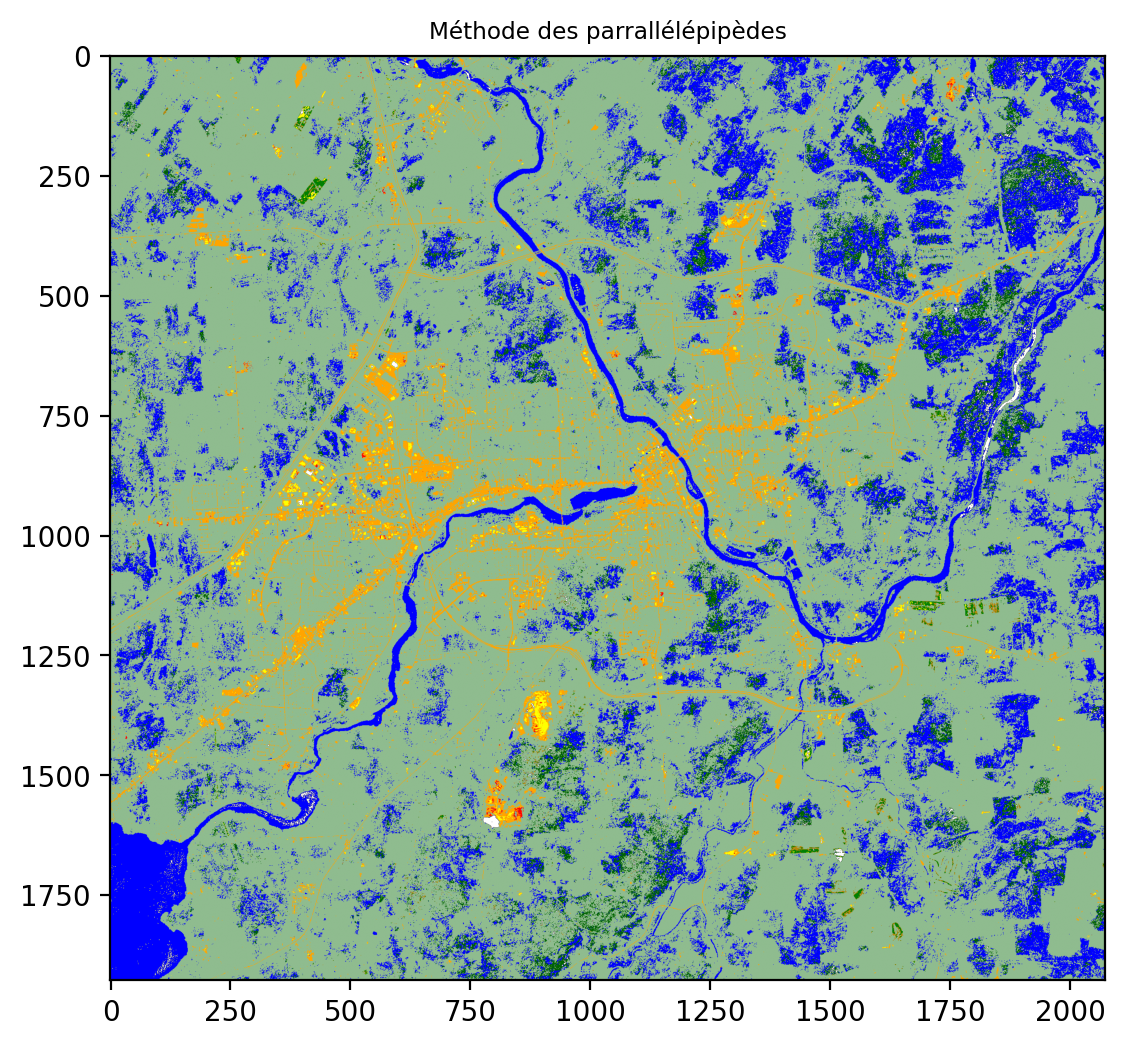
\includegraphics[width=6.14583in,height=4.05208in]{02-RehaussementVisualisationImages_files/figure-html/cell-23-output-1.png}
\caption{}
\end{figure}

Ainsi que les images:

\phantomsection\label{ba18ed4a}
\begin{figure}
\centering
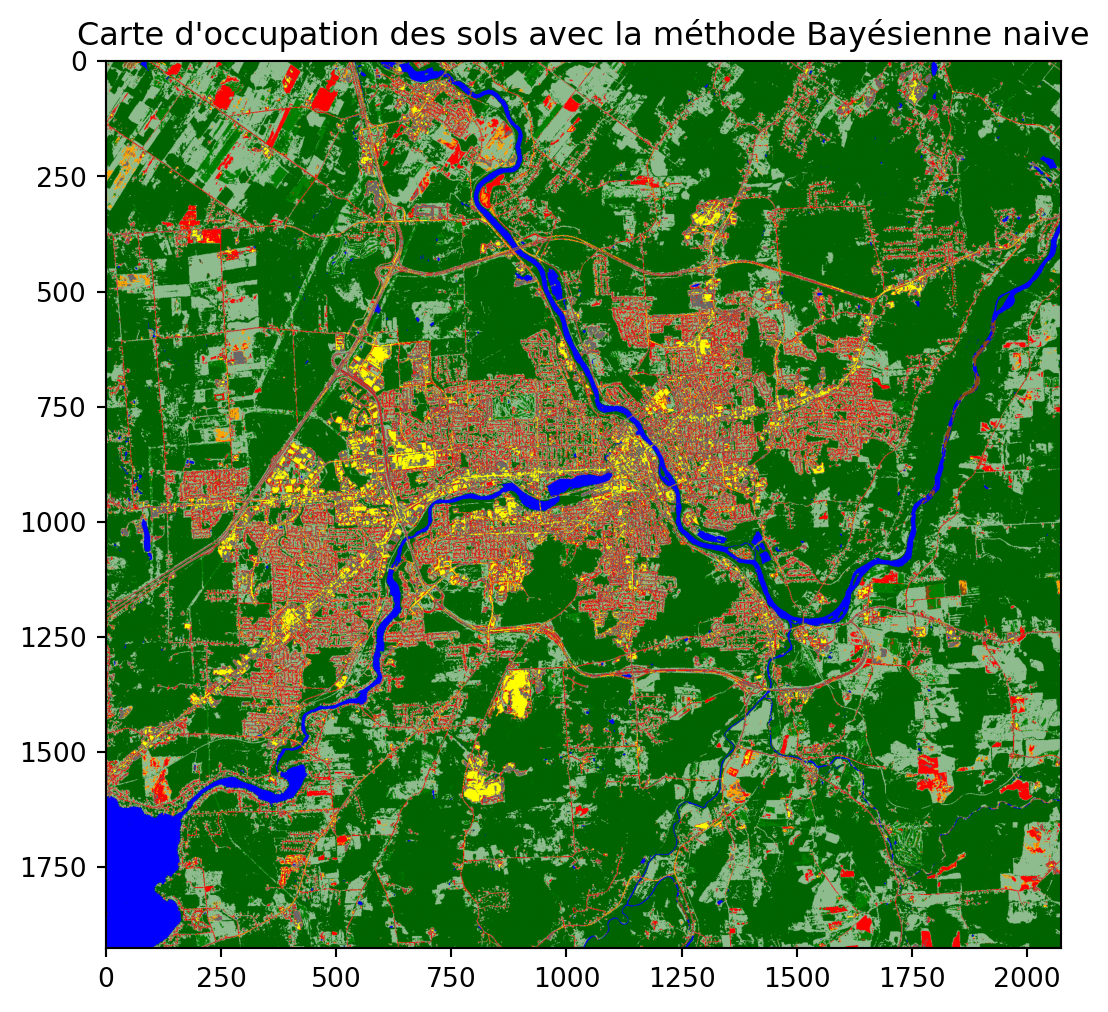
\includegraphics[width=6.14583in,height=5.04167in]{02-RehaussementVisualisationImages_files/figure-html/cell-24-output-1.png}
\caption{}
\end{figure}

\paragraph{\texorpdfstring{{3.3.3.2} Égalisation
d'histogramme}{3.3.3.2 Égalisation d'histogramme}}\label{uxe9galisation-dhistogramme}

L'égalisation d'histogramme consiste à modifier les valeurs des pixels
d'une image source de façon à ce que la distribution cumulée des valeurs
(CDF) deviennent similaire à celle d'une image cible. La CDF
(\emph{Cumulative Distribution Function}) est simplement la somme
cumulée des valeurs de l'histogramme:

{\textbackslash{[} CDF\_\{source\}(i)=
\textbackslash frac\{1\}\{K\}\textbackslash sum\_\{j=0\}\^{}\{j
\textbackslash leq i\} hist\_\{source\}(j) \textbackslash{]}} avec
{\textbackslash(K\textbackslash)} choisit de façon à ce que la dernière
valeur soit égale à 1
({\textbackslash(CDF\_\{source\}(i\_\{max\})=1\textbackslash)}). De la
même manière, {\textbackslash(CDF\_\{cible\}\textbackslash)} est la CDF
d'une image cible. La formule générale pour l'égalisation d'histogramme
est la suivante: {\textbackslash{[} j =
CDF\_\{cible\}\^{}\{-1\}(CDF\_\{source\}(i)) \textbackslash{]}}

On peut choisir {\textbackslash(CDF\_\{cible\}\textbackslash)} comme
correspondant à une image où chaque valeur de pixel est équiprobable
(d'où le terme \emph{égalisation}), ce qui veut dire
{\textbackslash(hist\_\{cible\}(j)=1/L\textbackslash)} avec
{\textbackslash(L\textbackslash)} égale au nombre de valeurs possibles
dans l'image (par exemple {\textbackslash(L=256\textbackslash)}).
{\textbackslash{[} j = L \textbackslash times CDF\_\{source\}(i)
\textbackslash{]}} On peut appliquer cette procédure sur l'image SAR en
dB de la façon suivante:

\phantomsection\label{fbb82e7a}
\phantomsection\label{cb26}
\begin{Shaded}
\begin{Highlighting}[]
\NormalTok{values}\OperatorTok{=}\NormalTok{ np.sort(np.log10(img\_SAR[}\DecValTok{0}\NormalTok{].data.flatten()))}
\NormalTok{cdf\_x}\OperatorTok{=}\NormalTok{ np.linspace(values[}\DecValTok{0}\NormalTok{], values[}\OperatorTok{{-}}\DecValTok{1}\NormalTok{], }\DecValTok{1000}\NormalTok{)}
\NormalTok{cdf\_source}\OperatorTok{=}\NormalTok{ np.interp(cdf\_x, values, np.arange(}\BuiltInTok{len}\NormalTok{(values))}\OperatorTok{/}\BuiltInTok{len}\NormalTok{(values)}\OperatorTok{*}\DecValTok{255}\NormalTok{)}
\NormalTok{values\_eq}\OperatorTok{=}\NormalTok{np.interp(np.log10(img\_SAR[}\DecValTok{0}\NormalTok{].data), cdf\_x, cdf\_source).astype(}\StringTok{\textquotesingle{}uint8\textquotesingle{}}\NormalTok{)}
\NormalTok{plt.imshow(values\_eq)}
\NormalTok{plt.axis(}\StringTok{\textquotesingle{}off\textquotesingle{}}\NormalTok{)}
\end{Highlighting}
\end{Shaded}

\begin{figure}
\centering
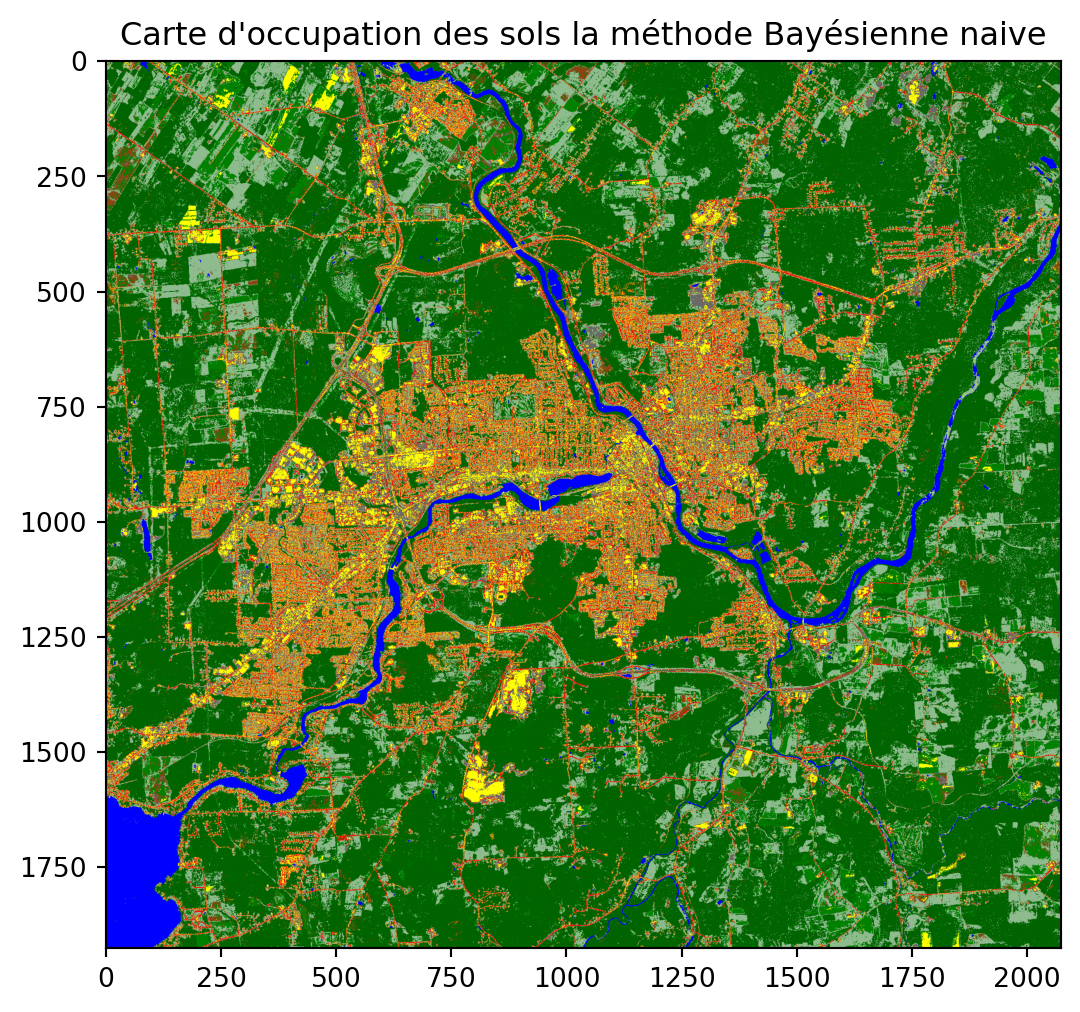
\includegraphics[width=5.60417in,height=4.21875in]{02-RehaussementVisualisationImages_files/figure-html/cell-25-output-1.png}
\caption{}
\end{figure}

\paragraph{\texorpdfstring{{3.3.3.3} Palettes de
couleur}{3.3.3.3 Palettes de couleur}}\label{palettes-de-couleur}

Les palettes de couleurs sont appliquées dynamiquement à l'affichage sur
une image à une seule bande. La librairie \texttt{matplotlib} contient
un nombre important de
\href{https://matplotlib.org/stable/users/explain/colors/colormaps.html}{palettes}.

\phantomsection\label{4f7723ee}
\phantomsection\label{cb27}
\begin{Shaded}
\begin{Highlighting}[]
\ImportTok{from}\NormalTok{ matplotlib }\ImportTok{import}\NormalTok{ colormaps}
\BuiltInTok{list}\NormalTok{(colormaps)}
\end{Highlighting}
\end{Shaded}

Voici quelques exemples ci-dessous, les valeurs de l'image doivent être
normalisées entre 0 et 1 ou entre 0 et 255 sinon les paramètres
\texttt{vmin} et \texttt{vmax} doivent être spécifiés. On peut observer
comment ces palettes révèlent les détails de l'image malgré une image
originalement très sombre.

\phantomsection\label{353a8b83}
\phantomsection\label{cb28}
\begin{Shaded}
\begin{Highlighting}[]
\NormalTok{fig, ax }\OperatorTok{=}\NormalTok{ plt.subplots(nrows}\OperatorTok{=}\DecValTok{2}\NormalTok{, ncols}\OperatorTok{=}\DecValTok{2}\NormalTok{, figsize}\OperatorTok{=}\NormalTok{(}\DecValTok{6}\NormalTok{, }\DecValTok{5}\NormalTok{), sharex}\OperatorTok{=}\VariableTok{True}\NormalTok{, sharey}\OperatorTok{=}\VariableTok{True}\NormalTok{)}
\NormalTok{[a.axis(}\StringTok{\textquotesingle{}off\textquotesingle{}}\NormalTok{) }\ControlFlowTok{for}\NormalTok{ a }\KeywordTok{in}\NormalTok{ ax.flatten()]}
\NormalTok{ax[}\DecValTok{0}\NormalTok{,}\DecValTok{0}\NormalTok{].imshow(img\_SAR[}\DecValTok{0}\NormalTok{].data, vmin}\OperatorTok{=}\NormalTok{percentiles[}\DecValTok{2}\NormalTok{], vmax}\OperatorTok{=}\NormalTok{percentiles[}\DecValTok{98}\NormalTok{], cmap}\OperatorTok{=}\StringTok{\textquotesingle{}jet\textquotesingle{}}\NormalTok{)}
\NormalTok{ax[}\DecValTok{0}\NormalTok{,}\DecValTok{0}\NormalTok{].set\_title(}\SpecialStringTok{f"jet"}\NormalTok{)}
\NormalTok{ax[}\DecValTok{0}\NormalTok{,}\DecValTok{1}\NormalTok{].imshow(img\_SAR[}\DecValTok{0}\NormalTok{].data, vmin}\OperatorTok{=}\NormalTok{percentiles[}\DecValTok{2}\NormalTok{], vmax}\OperatorTok{=}\NormalTok{percentiles[}\DecValTok{98}\NormalTok{], cmap}\OperatorTok{=}\StringTok{\textquotesingle{}hot\textquotesingle{}}\NormalTok{)}
\NormalTok{ax[}\DecValTok{0}\NormalTok{,}\DecValTok{1}\NormalTok{].set\_title(}\SpecialStringTok{f"hot"}\NormalTok{)}
\NormalTok{ax[}\DecValTok{1}\NormalTok{,}\DecValTok{0}\NormalTok{].imshow(img\_SAR[}\DecValTok{0}\NormalTok{].data, vmin}\OperatorTok{=}\NormalTok{percentiles[}\DecValTok{2}\NormalTok{], vmax}\OperatorTok{=}\NormalTok{percentiles[}\DecValTok{98}\NormalTok{], cmap}\OperatorTok{=}\StringTok{\textquotesingle{}hsv\textquotesingle{}}\NormalTok{)}
\NormalTok{ax[}\DecValTok{1}\NormalTok{,}\DecValTok{0}\NormalTok{].set\_title(}\SpecialStringTok{f"hsv"}\NormalTok{)}
\NormalTok{ax[}\DecValTok{1}\NormalTok{,}\DecValTok{1}\NormalTok{].imshow(img\_SAR[}\DecValTok{0}\NormalTok{].data, vmin}\OperatorTok{=}\NormalTok{percentiles[}\DecValTok{2}\NormalTok{], vmax}\OperatorTok{=}\NormalTok{percentiles[}\DecValTok{98}\NormalTok{], cmap}\OperatorTok{=}\StringTok{\textquotesingle{}terrain\textquotesingle{}}\NormalTok{)}
\NormalTok{ax[}\DecValTok{1}\NormalTok{,}\DecValTok{1}\NormalTok{].set\_title(}\SpecialStringTok{f"terrain"}\NormalTok{)}
\NormalTok{plt.tight\_layout()}
\end{Highlighting}
\end{Shaded}

\begin{figure}
\centering
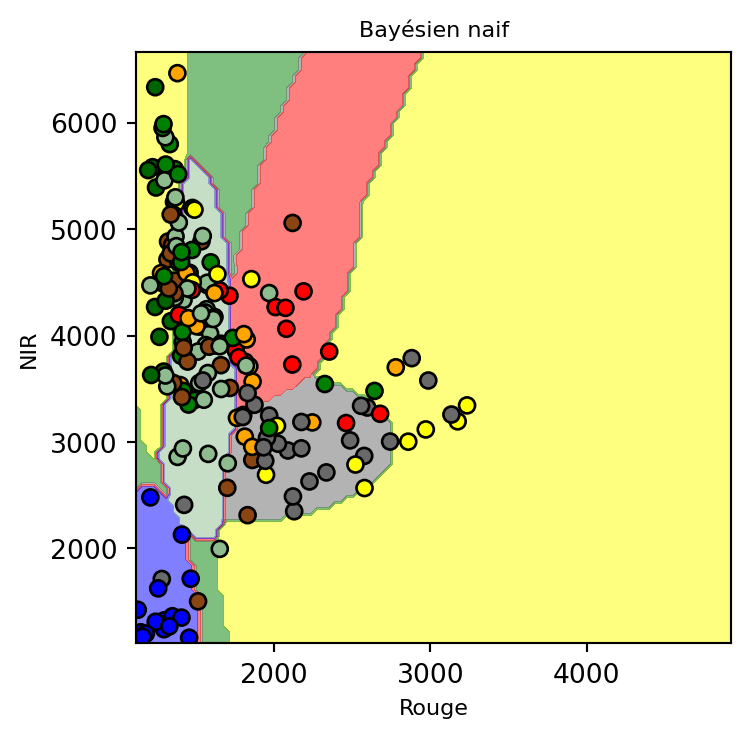
\includegraphics[width=6.14583in,height=5.04167in]{02-RehaussementVisualisationImages_files/figure-html/cell-27-output-1.png}
\caption{}
\end{figure}

Il peut être utile d'ajouter une barre de couleurs afin d'indiquer la
correspondance entre les couleurs et les valeurs numériques:

\phantomsection\label{5cd60403}
\phantomsection\label{cb29}
\begin{Shaded}
\begin{Highlighting}[]
\ImportTok{import}\NormalTok{ matplotlib }\ImportTok{as}\NormalTok{ mpl}
\NormalTok{fig, ax }\OperatorTok{=}\NormalTok{ plt.subplots(figsize}\OperatorTok{=}\NormalTok{(}\DecValTok{6}\NormalTok{, }\DecValTok{6}\NormalTok{))}
\NormalTok{cmap}\OperatorTok{=}\NormalTok{ mpl.colormaps.get\_cmap(}\StringTok{\textquotesingle{}jet\textquotesingle{}}\NormalTok{).with\_extremes(under}\OperatorTok{=}\StringTok{\textquotesingle{}white\textquotesingle{}}\NormalTok{, over}\OperatorTok{=}\StringTok{\textquotesingle{}magenta\textquotesingle{}}\NormalTok{)}
\NormalTok{h}\OperatorTok{=}\NormalTok{plt.imshow(img\_SAR[}\DecValTok{0}\NormalTok{].data, norm}\OperatorTok{=}\NormalTok{mpl.colors.LogNorm(vmin}\OperatorTok{=}\NormalTok{percentiles[}\DecValTok{2}\NormalTok{], vmax}\OperatorTok{=}\NormalTok{percentiles[}\DecValTok{98}\NormalTok{]),}
\NormalTok{                   cmap}\OperatorTok{=}\NormalTok{cmap)}
\NormalTok{fig.colorbar(h, ax}\OperatorTok{=}\NormalTok{ax,  orientation}\OperatorTok{=}\StringTok{\textquotesingle{}horizontal\textquotesingle{}}\NormalTok{, label}\OperatorTok{=}\StringTok{"Intensité"}\NormalTok{, extend}\OperatorTok{=}\StringTok{\textquotesingle{}both\textquotesingle{}}\NormalTok{)}
\NormalTok{ax.axis(}\StringTok{\textquotesingle{}off\textquotesingle{}}\NormalTok{) }
\end{Highlighting}
\end{Shaded}

\begin{figure}
\centering
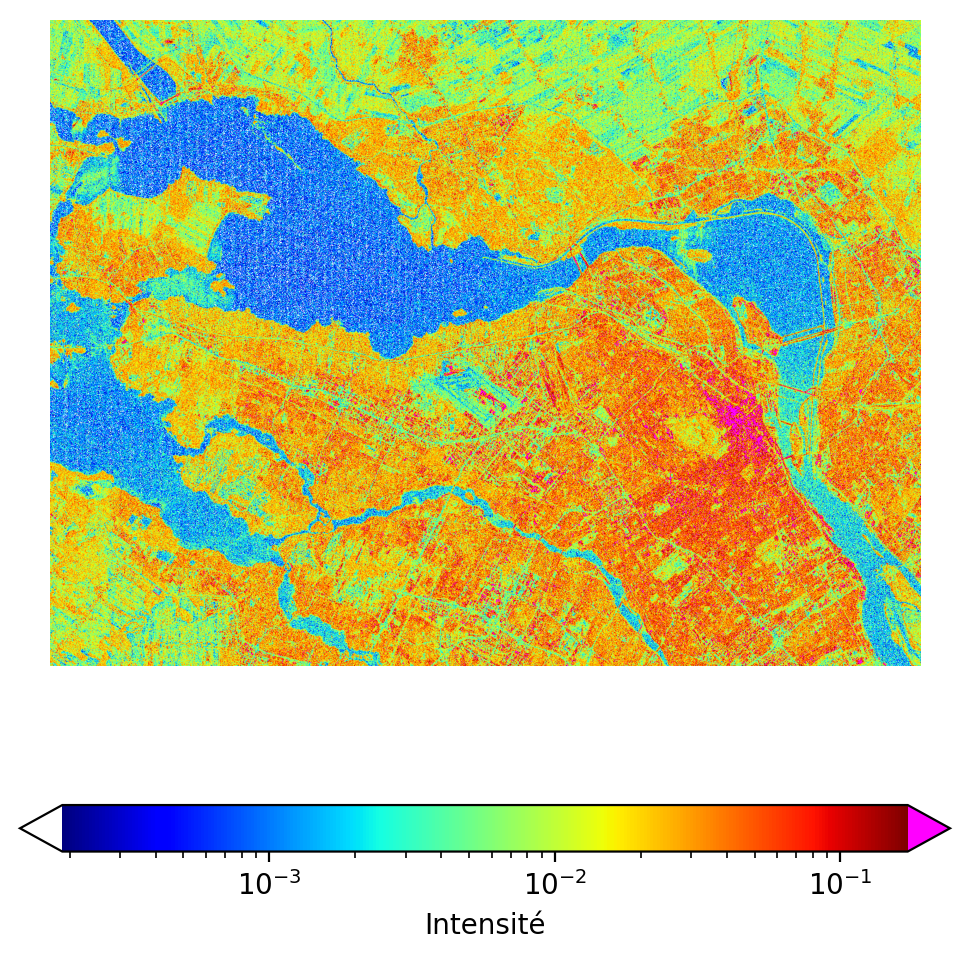
\includegraphics[width=5.05208in,height=5in]{02-RehaussementVisualisationImages_files/figure-html/cell-28-output-1.png}
\caption{}
\end{figure}

\subsubsection{\texorpdfstring{{3.3.4} Composés
couleurs}{3.3.4 Composés couleurs}}\label{composuxe9s-couleurs}

Le système visuel humain est sensible seulement à la partie visible du
spectre électromagnétique qui compose les couleurs de l'arc-en-ciel du
bleu au rouge. L'ensemble des couleurs du spectre visible peut être
obtenu à partir du mélange de trois couleurs primaires (rouge, vert et
bleu). Ce système de décomposition à trois couleurs est à la base de la
plupart des systèmes de visualisation ou de représentation de
l'information de couleur. Si on prend le cas des images Sentinel-2, 12
bandes sont disponibles, plusieurs composés couleurs sont donc possibles
(voir le site de
\href{https://custom-scripts.sentinel-hub.com/custom-scripts/sentinel-2/composites/}{Copernicus}).
Voici quelques exemples possibles, chaque composé mettant en valeur des
propriétés différentes de la surface.

\phantomsection\label{581e6675}
\phantomsection\label{cb30}
\begin{Shaded}
\begin{Highlighting}[]
\ImportTok{import}\NormalTok{ rioxarray }\ImportTok{as}\NormalTok{ rxr}
\NormalTok{fig, ax}\OperatorTok{=}\NormalTok{ plt.subplots(nrows}\OperatorTok{=}\DecValTok{2}\NormalTok{, ncols}\OperatorTok{=} \DecValTok{2}\NormalTok{, figsize}\OperatorTok{=}\NormalTok{(}\DecValTok{8}\NormalTok{, }\DecValTok{6}\NormalTok{), sharex}\OperatorTok{=}\VariableTok{True}\NormalTok{, sharey}\OperatorTok{=}\VariableTok{True}\NormalTok{)}
\NormalTok{img\_s2.sel(band}\OperatorTok{=}\NormalTok{[}\DecValTok{4}\NormalTok{,}\DecValTok{3}\NormalTok{,}\DecValTok{2}\NormalTok{]).plot.imshow(vmin}\OperatorTok{=}\DecValTok{86}\NormalTok{, vmax}\OperatorTok{=}\DecValTok{4000}\NormalTok{, ax}\OperatorTok{=}\NormalTok{ax[}\DecValTok{0}\NormalTok{,}\DecValTok{0}\NormalTok{])}
\NormalTok{ax[}\DecValTok{0}\NormalTok{,}\DecValTok{0}\NormalTok{].set\_title(}\StringTok{\textquotesingle{}RVB\textquotesingle{}}\NormalTok{)}
\NormalTok{img\_s2.sel(band}\OperatorTok{=}\NormalTok{[}\DecValTok{8}\NormalTok{,}\DecValTok{3}\NormalTok{,}\DecValTok{2}\NormalTok{]).plot.imshow(vmin}\OperatorTok{=}\DecValTok{86}\NormalTok{, vmax}\OperatorTok{=}\DecValTok{4000}\NormalTok{, ax}\OperatorTok{=}\NormalTok{ax[}\DecValTok{0}\NormalTok{,}\DecValTok{1}\NormalTok{])}
\NormalTok{ax[}\DecValTok{0}\NormalTok{,}\DecValTok{1}\NormalTok{].set\_title(}\StringTok{\textquotesingle{}NIR,V,B\textquotesingle{}}\NormalTok{)}
\NormalTok{img\_s2.sel(band}\OperatorTok{=}\NormalTok{[}\DecValTok{12}\NormalTok{,}\DecValTok{8}\NormalTok{,}\DecValTok{4}\NormalTok{]).plot.imshow(vmin}\OperatorTok{=}\DecValTok{86}\NormalTok{, vmax}\OperatorTok{=}\DecValTok{4000}\NormalTok{, ax}\OperatorTok{=}\NormalTok{ax[}\DecValTok{1}\NormalTok{,}\DecValTok{0}\NormalTok{])}
\NormalTok{ax[}\DecValTok{1}\NormalTok{,}\DecValTok{0}\NormalTok{].set\_title(}\StringTok{\textquotesingle{}SWIR2,NIR,R\textquotesingle{}}\NormalTok{)}
\NormalTok{img\_s2.sel(band}\OperatorTok{=}\NormalTok{[}\DecValTok{12}\NormalTok{,}\DecValTok{11}\NormalTok{,}\DecValTok{4}\NormalTok{]).plot.imshow(vmin}\OperatorTok{=}\DecValTok{86}\NormalTok{, vmax}\OperatorTok{=}\DecValTok{4000}\NormalTok{, ax}\OperatorTok{=}\NormalTok{ax[}\DecValTok{1}\NormalTok{,}\DecValTok{1}\NormalTok{])}
\NormalTok{ax[}\DecValTok{1}\NormalTok{,}\DecValTok{1}\NormalTok{].set\_title(}\StringTok{\textquotesingle{}SWIR2,SWIR1,NIR\textquotesingle{}}\NormalTok{)}
\NormalTok{plt.tight\_layout()}
\NormalTok{plt.show()}
\end{Highlighting}
\end{Shaded}

\begin{figure}
\centering
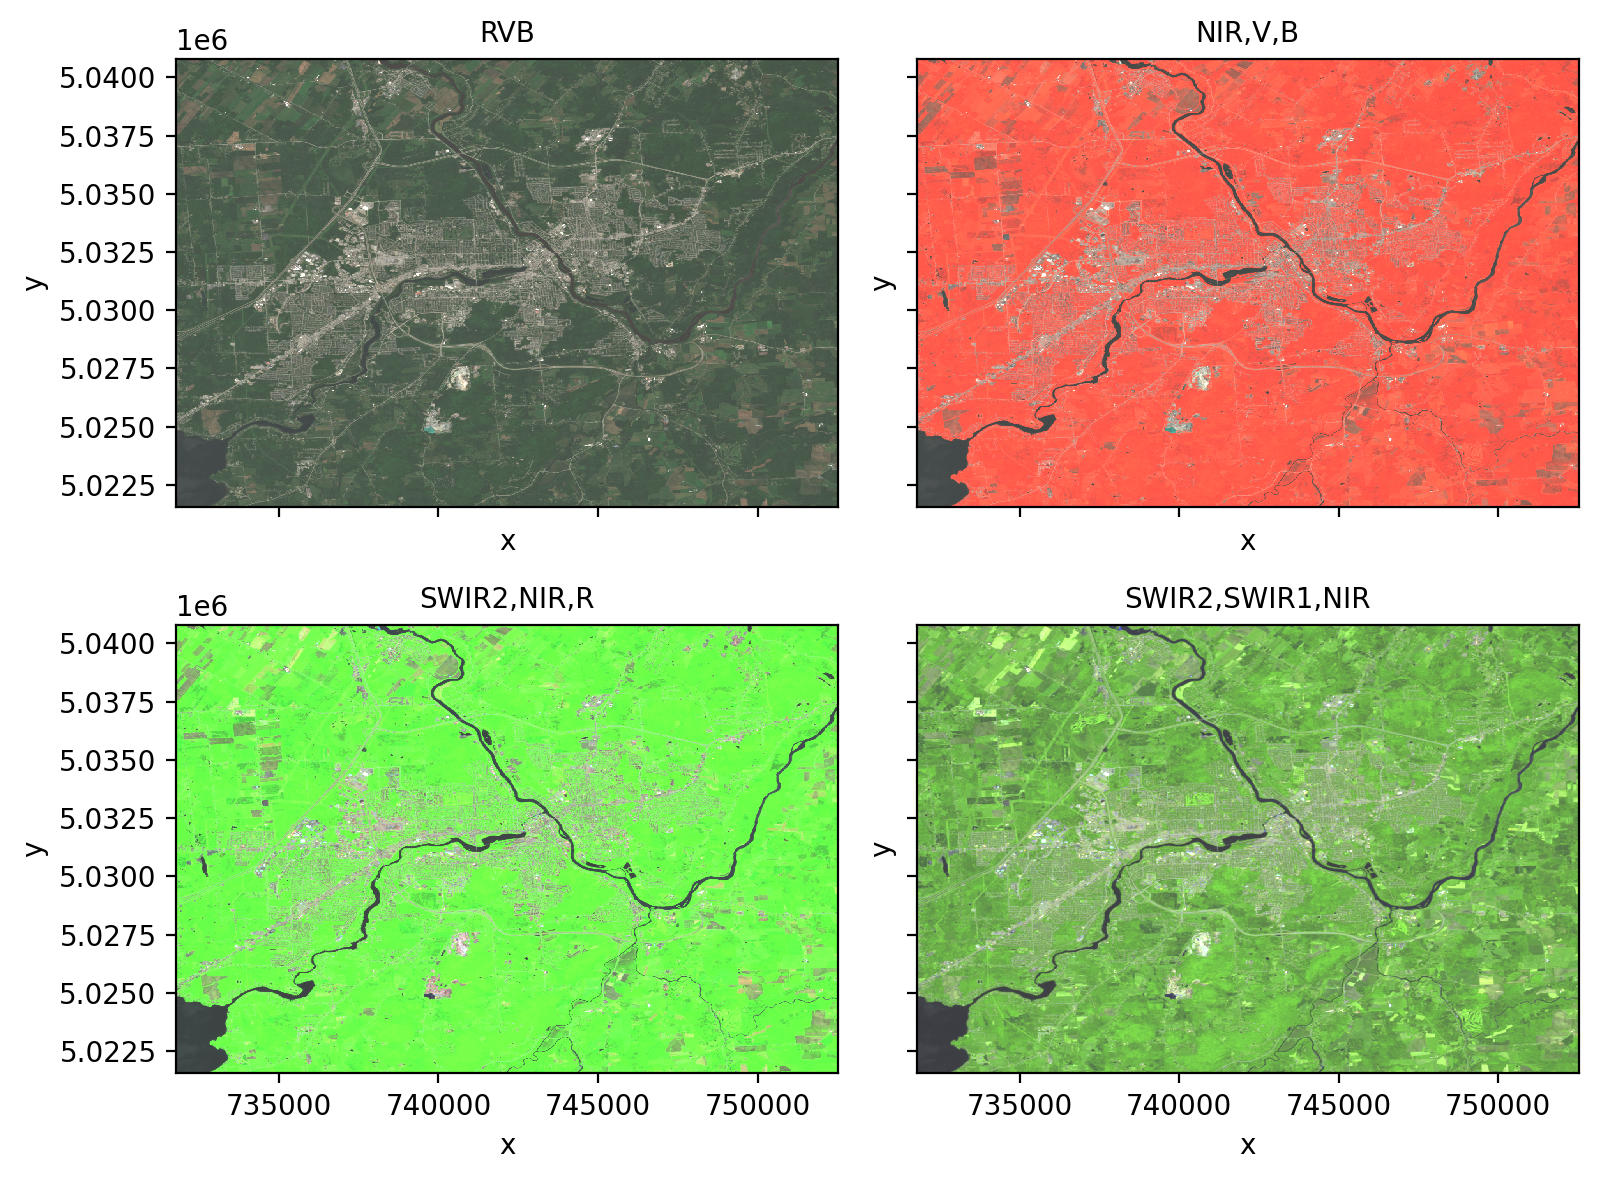
\includegraphics[width=8.32292in,height=6.14583in]{02-RehaussementVisualisationImages_files/figure-html/cell-29-output-1.png}
\caption{}
\end{figure}

\end{document}
